%% chapters/04-diagnostik.tex
%% Bab IV — Deteksi Kerusakan \emph{Bearing}: Metodologi dan Hasil
%% Sumber utama:
%%   Conference 1 — SVM/LR + SHAP KernelExplainer (§IV.2, §IV.7)
%%   Conference 2 — DT/RF/XGBoost + SHAP TreeExplainer (§IV.3, §IV.8)
%%   Journal 1    — WDCNN + SHAP DeepExplainer + FSM (§IV.4–IV.6, §IV.9–IV.14)
%% Fase D — dibuat sesuai writings/dissertation-outline.md §Bab IV

\chapter{Deteksi Kerusakan \emph{Bearing}: Metodologi dan Hasil}
\label{bab:diagnostik}

Bab ini menyajikan \textcolor{blue}{komponen diagnostik} secara \emph{end-to-end}: dari perancangan
metodologi \emph{benchmark} lintas tiga kelompok algoritma hingga analisis
hasil, validasi interpretabilitas, dan sintesis lintas kelompok.
Sumber empiris utama terdiri atas tiga karya yang masing-masing merepresentasikan
satu kelompok algoritma: \citetitb{TotoSuharto2024Conf1SVM} untuk model
berbasis kernel (SVM dan Regresi Logistik), \citetitb{TotoSuharto2024Conf2Tree}
untuk algoritma berbasis pohon (DT, RF, XGBoost), dan
\citetitb{TotoSuharto2025Journal1FSM} untuk arsitektur jaringan dalam (WDCNN)
beserta formalisasi \emph{Fault Signature Maps} (FSM).

Fondasi bersama bab ini, yaitu dataset CWRU, prosedur praproses sinyal, vektor
fitur HI~36-D, metrik evaluasi diagnostik dan FSM, serta infrastruktur
komputasi, telah diuraikan pada Bab~\ref{bab:metodologi-umum}.
Bab ini tidak mengulang uraian tersebut, melainkan mengembangkan metodologi
spesifik tiap kelompok dan menyajikan hasil eksperimen beserta interpretasinya.
Subbab §IV.1 s.d.\ §IV.6 membahas metodologi; subbab §IV.7 s.d.\ §IV.14
membahas hasil dan analisis.

% =================================================================
\section{Pipeline Diagnostik CWRU: Ikhtisar}
\label{sec:bab4_pipeline}
% =================================================================

Jalur diagnostik pada penelitian ini menggunakan dataset CWRU sebagai
sumber data tunggal dan merancang dua alur paralel sesuai representasi
input yang sesuai per kelompok model.
Alur pertama mengekstraksi vektor fitur HI~36-D dari setiap segmen sinyal
sebelum memasukkannya ke model berbasis kernel dan algoritma berbasis pohon,
karena kedua kelompok model tersebut beroperasi pada ruang fitur berdimensi tetap.
Alur kedua melewatkan sinyal mentah 2.048 titik secara langsung ke WDCNN,
yang merancang lapisan konvolusi pertamanya sebagai ekstraktor frekuensi
adaptif otomatis tanpa rekayasa fitur manual.

Gambar~\ref{fig:bab4_pipeline_diagnostik} mengilustrasikan pipeline dua
alur ini beserta modul \emph{Explainable AI} (SHAP) yang menyertai setiap
kelompok.
Pada alur fitur, SHAP \emph{KernelExplainer} (untuk SVM/LR) dan SHAP
\emph{TreeExplainer} (untuk DT/RF/XGBoost) menghasilkan atribusi pada
ruang fitur HI~36-D.
Pada alur sinyal, SHAP \emph{DeepExplainer} menghasilkan atribusi langsung
pada 2.048 posisi sinyal mentah, yang kemudian diagregasi menjadi FSM
sebagai \emph{fingerprint} per kelas kerusakan.

\begin{figure}[ht]
\centering
\resizebox{\textwidth}{!}{%
\begin{tikzpicture}[
    node distance = 0.4cm and 0.9cm,
    ds/.style   = {rectangle, rounded corners=3pt, draw, thick, fill=gray!15,
                   align=center, minimum height=0.80cm, minimum width=2.4cm,
                   font=\small},
    ker/.style  = {rectangle, rounded corners=3pt, draw, thick, fill=blue!10,
                   align=center, minimum height=0.80cm, minimum width=2.6cm,
                   font=\small},
    deep/.style = {rectangle, rounded corners=3pt, draw, thick, fill=green!10,
                   align=center, minimum height=0.80cm, minimum width=2.6cm,
                   font=\small},
    xai/.style  = {rectangle, rounded corners=3pt, draw, thick, fill=yellow!15,
                   align=center, minimum height=0.80cm, minimum width=2.8cm,
                   font=\small},
    outnode/.style = {rectangle, rounded corners=3pt, draw, thick, fill=orange!15,
                   align=center, minimum height=0.80cm, minimum width=2.4cm,
                   font=\small},
    arr/.style  = {-{Stealth[length=5pt]}, thick},
  ]
  %% Sumber data
  \node[ds] (cwru) {CWRU\\{\scriptsize 2.048 titik, 10 kelas}};

  %% Alur 1 — Fitur HI
  \node[ker, above right=0.8cm and 1.0cm of cwru] (feat)
       {HI 36-D\\{\scriptsize 9 waktu + 9 frekuensi $\times$ 2 kanal}};
  \node[ker, right=0.9cm of feat] (kertree)
       {Kernel/Tree\\{\scriptsize SVM, LR, DT, RF, XGB}};
  \node[xai, right=0.9cm of kertree] (shapft)
       {SHAP\\{\scriptsize Kernel/TreeExplainer}};
  \node[outnode, right=0.9cm of shapft] (rankf)
       {Ranking fitur\\{\scriptsize global \& per kelas}};

  \draw[arr] (cwru.north east) |- (feat.west);
  \draw[arr] (feat)    -- (kertree);
  \draw[arr] (kertree) -- (shapft);
  \draw[arr] (shapft)  -- (rankf);

  %% Alur 2 — Sinyal mentah
  \node[deep, below right=0.8cm and 1.0cm of cwru] (raw)
       {Sinyal mentah\\{\scriptsize $\mathbb{R}^{2048}$, tanpa ekstraksi}};
  \node[deep, right=0.9cm of raw] (wdcnn)
       {WDCNN\\{\scriptsize kernel-1 = 64, BN, dropout}};
  \node[xai, right=0.9cm of wdcnn] (shapd)
       {SHAP\\{\scriptsize DeepExplainer}};
  \node[outnode, right=0.9cm of shapd] (fsm)
       {FSM\\{\scriptsize \emph{fingerprint} 2.048 posisi}};

  \draw[arr] (cwru.south east) |- (raw.west);
  \draw[arr] (raw)   -- (wdcnn);
  \draw[arr] (wdcnn) -- (shapd);
  \draw[arr] (shapd) -- (fsm);

  %% Label alur
  \node[font=\scriptsize\bfseries, text=blue!70!black,
        above=0.15cm of feat] {Alur 1 — Kernel/Tree};
  \node[font=\scriptsize\bfseries, text=green!60!black,
        below=0.15cm of raw] {Alur 2 — Deep (WDCNN)};

\end{tikzpicture}%
}
\caption{Pipeline diagnostik CWRU dua alur. Alur~1 (biru) mengekstraksi vektor
         fitur HI~36-D sebelum melatih model kernel atau \emph{tree}; modul
         SHAP \emph{KernelExplainer} dan \emph{TreeExplainer} menghasilkan
         atribusi di ruang fitur. Alur~2 (hijau) memasukkan sinyal mentah
         2.048 titik langsung ke WDCNN; SHAP \emph{DeepExplainer} menghasilkan
         atribusi resolusi sinyal yang diagregasi menjadi FSM.}
\label{fig:bab4_pipeline_diagnostik}
\end{figure}

Pemilihan dua alur paralel mencerminkan perbedaan mendasar dalam desain
model, bukan sekadar perbedaan implementasi.
Model berbasis kernel dan algoritma berbasis pohon dirancang untuk beroperasi
pada perangkat dengan sumber daya terbatas (\emph{edge} IoT) karena membutuhkan
lebih sedikit memori dan komputasi inferensi dibandingkan jaringan dalam.
WDCNN, di sisi lain, dioptimalkan untuk akurasi maksimum dengan interpretabilitas
level sinyal yang lebih kaya, yaitu kemampuan yang tidak tersedia pada model
berbasis kernel maupun algoritma berbasis pohon ketika beroperasi pada
representasi sinyal mentah.
Perbandingan lintas kedua alur pada §IV.14 mengungkap implikasi desain
sistem PdM multi-tier yang lebih luas.

% =================================================================
\section{Benchmark Model Berbasis Kernel: SVM dan Regresi Logistik}
\label{sec:bab4_kernel}
% =================================================================

Dua model berbasis kernel dievaluasi: \emph{Support Vector Machine} (SVM)
dengan kernel RBF dan Regresi Logistik (\emph{Logistic Regression}, LR)
dengan skema \emph{one-vs-rest} untuk klasifikasi sepuluh kelas.
Kedua model beroperasi pada vektor fitur HI~36-D yang diekstraksi dari
sinyal CWRU sebagaimana diuraikan pada
Subbab~\ref{subsec:bab3_hi36d} \citetitb{TotoSuharto2024Conf1SVM}.

\subsection{Ekstraksi Fitur untuk Model Berbasis Kernel}
\label{subsec:bab4_kernel_fitur}

Dari setiap segmen sinyal CWRU sepanjang 2.048 titik, diekstraksi
\textbf{sembilan fitur domain waktu} per kanal akselerometer:
(1) nilai RMS, (2) kurtosis, (3) \emph{crest factor},
(4) \emph{peak-to-peak}, (5) \emph{skewness}, (6) deviasi standar,
(7) mean, (8) variansi, dan (9) \emph{median absolute deviation} (MAD).
Selain itu, diekstraksi \textbf{sembilan fitur domain frekuensi} per kanal:
sentroid spektral, entropi spektral, dan tujuh nilai energi pita frekuensi
yang mencakup pita sekitar BPFO, BPFI, BSF, FTF beserta harmonik pertamanya.
Dengan dua kanal (drive-end dan fan-end), total dimensi vektor HI per segmen
adalah $9 \times 2 + 9 \times 2 = 36$, selaras dengan definisi lengkap
pada Lampiran~\ref{lamp:fitur}.

Setelah ekstraksi, vektor HI~36-D dinormalisasi ulang menggunakan Z-score
berbasis statistik \emph{training set} (terpisah dari normalisasi sinyal
mentah pada Persamaan~\ref{eq:bab3_zscore}), sehingga setiap fitur memiliki
distribusi zero-mean unit-variance pada ruang input model.
Normalisasi ini bersifat wajib untuk SVM-RBF agar jarak antar sampel dalam
ruang kernel tidak didominasi fitur dengan skala besar.

\subsection{Konfigurasi SVM-RBF}
\label{subsec:bab4_svm_config}

SVM dengan kernel RBF dilatih pada \emph{training set} CWRU menggunakan
dua hiperparameter utama yang dioptimasi melalui GridSearchCV:
$C \in \{0{,}1;\; 1;\; 10;\; 100\}$ dan
$\gamma \in \{\text{scale},\; \text{auto},\; 0{,}01;\; 0{,}1\}$.
Parameter \texttt{class\_weight=\textquotesingle balanced\textquotesingle}
ditetapkan untuk memastikan kelas-kelas yang seimbang ditangani secara adil.
Pembagian data menggunakan stratified 80/20 dengan \texttt{random\_state}
tetap, dan optimasi hiperparameter dilakukan melalui stratified 5-fold
\emph{cross-validation} pada \emph{training set} sebelum evaluasi pada
\emph{test set}.

\subsection{Konfigurasi Regresi Logistik}
\label{subsec:bab4_lr_config}

Regresi Logistik dikonfigurasi dengan skema \emph{one-vs-rest} (OvR) untuk
menghasilkan prediksi sepuluh kelas secara langsung dari satu model.
Parameter regulasi $C \in \{0{,}1;\; 1;\; 10\}$ dioptimasi melalui
GridSearchCV identik dengan SVM.
Solver \texttt{lbfgs} digunakan karena lebih efisien untuk dataset ukuran
sedang dengan fitur kontinu.
Nilai $C$ optimal yang lebih rendah dibandingkan SVM mencerminkan sifat LR
yang lebih sensitif terhadap regularisasi untuk mencegah \emph{overfitting}
pada batas keputusan linear.

% =================================================================
\section{Benchmark Algoritma Berbasis Pohon: DT, RF, dan XGBoost}
\label{sec:bab4_tree}
% =================================================================

Tiga algoritma berbasis pohon dievaluasi untuk merepresentasikan tiga
tingkat kompleksitas yang berbeda: \emph{Decision Tree} (DT) sebagai model
tunggal yang dapat divisualisasikan, \emph{Random Forest} (RF) sebagai
agregasi \emph{bagging}, dan XGBoost sebagai \emph{gradient boosting} dengan
regularisasi \citetitb{TotoSuharto2024Conf2Tree}.
Ketiga model beroperasi pada vektor fitur HI~36-D yang sama dengan model
berbasis kernel, mengikuti protokol \emph{split} dan normalisasi identik.

\subsection{Konfigurasi Decision Tree}
\label{subsec:bab4_dt_config}

DT dilatih dengan kriteria pemisahan Gini dan dibatasi kedalaman maksimum
(\texttt{max\_depth}) serta jumlah minimum sampel per daun
(\texttt{min\_samples\_leaf}) yang dioptimasi melalui GridSearchCV.
DT dipilih bukan karena performa tertingginya, melainkan karena interpretabilitas
strukturalnya yang paling tinggi di antara ketiga model: setiap keputusan
klasifikasi dapat ditelusuri melalui aturan \texttt{if-then} yang eksplisit.
Peran DT dalam \emph{benchmark} adalah menetapkan batas bawah yang dapat
diinterpretasi sepenuhnya tanpa modul SHAP.

\subsection{Konfigurasi Random Forest}
\label{subsec:bab4_rf_config}

RF menggunakan 100 pohon (\texttt{n\_estimators=100}) dengan kedalaman
maksimum 20 (\texttt{max\_depth=20}) dan pemilihan fitur acak sebesar
$\sqrt{36} \approx 6$ fitur per pemisahan (\texttt{max\_features=\textquotesingle sqrt\textquotesingle}).
\emph{Bagging} atas 100 pohon mereduksi variansi prediksi secara signifikan
dibandingkan DT tunggal, sehingga RF umumnya menghasilkan akurasi lebih
tinggi dengan biaya komputasi yang jauh lebih besar.
Bootstrap sampling (\texttt{bootstrap=True}) diterapkan agar setiap pohon
dilatih pada subset acak dari \emph{training set}.

\subsection{Konfigurasi XGBoost}
\label{subsec:bab4_xgb_config}

XGBoost dikonfigurasi dengan \texttt{n\_estimators=150},
\texttt{learning\_rate=0{,}05}, \texttt{max\_depth=6}, dan
\texttt{reg\_lambda=1{,}0} (regularisasi L2) untuk mengendalikan
\emph{overfitting}.
Satu aspek teknis penting: XGBoost mengharuskan label kelas berupa bilangan
bulat non-negatif (0 s.d.\ 9), sehingga diperlukan \emph{label encoding}
dari representasi string ke representasi integer sebelum pelatihan.
Transformasi ini bersifat deterministik dan tidak memengaruhi semantik
kelas; panduan lengkap implementasi tersedia di Lampiran~F.

% =================================================================
\section{Arsitektur Deep: WDCNN}
\label{sec:bab4_wdcnn}
% =================================================================

\emph{Wide-Deep Convolutional Neural Network} (WDCNN) merupakan arsitektur
jaringan konvolusi 1D yang dirancang khusus untuk klasifikasi kerusakan
\emph{bearing} dari sinyal mentah \citetitb{Zhang2017WDCNN}.
Arsitektur ini menggunakan lapisan konvolusi pertama berkernel lebar untuk
menangkap informasi frekuensi secara adaptif tanpa ekstraksi fitur manual,
diikuti blok konvolusi berkernel sempit untuk mempelajari representasi
hierarki yang lebih dalam.

\subsection{Detail Arsitektur WDCNN}
\label{subsec:bab4_wdcnn_detail}

Input model berupa sinyal mentah ternormalisasi berdimensi $1 \times 2048$
(satu kanal, 2.048 titik).
Lapisan pertama menggunakan kernel berukuran 64 dengan \emph{stride} 16,
menghasilkan peta aktivasi berdimensi $\lceil 2048/16 \rceil = 128$ dengan
jumlah filter tertentu; pilihan ukuran kernel 64 dan \emph{stride} 16 dirancang
agar satu jendela reseptif mencakup seluruh perioda impuls tipikal cacat
\emph{bearing} pada 48~kHz.
Lapisan konvolusi kedua hingga kelima menggunakan kernel berukuran 3 dengan
\emph{Batch Normalization} (BN), MaxPooling, dan fungsi aktivasi ReLU untuk
membangun representasi hierarki yang progresif.

Setelah blok konvolusi, dua lapisan \emph{fully connected} (FC) dengan 100
neuron masing-masing dan \emph{dropout rate} 0,5 ditempatkan sebelum lapisan
klasifikasi.
Lapisan keluaran menggunakan softmax dengan 10 unit sesuai dengan jumlah
kelas kerusakan CWRU.
Total parameter model mencapai \textasciitilde 60.710, termasuk bobot
lapisan konvolusi dan FC.
Tabel lengkap arsitektur per lapisan tersedia di Lampiran~G.

\subsection{Tiga Varian Ablasi}
\label{subsec:bab4_wdcnn_ablasi}

Tiga varian arsitektur digunakan untuk studi ablasi yang menjadi fondasi
Novelti~N2:

\begin{enumerate}
  \item \textbf{Varian A (Baseline):} WDCNN penuh dengan kernel pertama
        berukuran 64 dan \emph{Batch Normalization} aktif pada semua blok
        konvolusi. Varian ini merepresentasikan konfigurasi referensi
        \citetitb{Zhang2017WDCNN}.
  \item \textbf{Varian B (Kernel Sempit):} Ukuran kernel pertama diperkecil
        dari 64 ke 3 \textcolor{blue}{(\emph{stride} 16 menjadi 1)},
        menyamakan dengan kernel blok lainnya. Tujuan ablasi
        ini adalah menguji peran kernel lebar dalam pemrosesan frekuensi.
        \textcolor{blue}{Justru jumlah parameter melonjak sebesar faktor
        $7{,}3\times$ (dari 60.710 menjadi 443.734) karena hilangnya
        reduksi dimensi implisit oleh \emph{stride} lebar membuat peta fitur
        beresolusi penuh dan memerlukan bank filter yang jauh lebih besar.}
  \item \textbf{Varian C (Tanpa BatchNorm):} Arsitektur identik dengan
        Varian A, tetapi semua lapisan \emph{Batch Normalization} dihapus.
        Tujuan ablasi ini adalah menguji hipotesis bahwa BN menekan
        diskriminabilitas FSM, temuan yang menjadi inti Novelti~N2.
\end{enumerate}

\subsection{Protokol Pelatihan WDCNN}
\label{subsec:bab4_wdcnn_training}

Pelatihan menggunakan optimizer Adam dengan \emph{learning rate} awal 0,001
dan penjadwal \emph{Step Learning Rate} (StepLR, $\gamma = 0{,}5$, langkah
setiap 20 \emph{epoch}).
Fungsi \emph{loss} adalah \emph{CrossEntropyLoss} standar tanpa bobot kelas
(kelas CWRU seimbang 75 sampel per kelas pada \emph{test set}).
\emph{Early stopping} dengan kesabaran 15 \emph{epoch} diaktifkan berdasarkan
akurasi validasi, dan \emph{checkpoint} terbaik disimpan untuk evaluasi
akhir pada \emph{test set}.
Detail hiperparameter lengkap tersedia di Lampiran~G.

% =================================================================
\section{Analisis SHAP per Kelompok Algoritma}
\label{sec:bab4_shap}
% =================================================================

Setiap kelompok algoritma menggunakan varian SHAP yang berbeda sesuai dengan
struktur modelnya.
Pemilihan varian ini bukan sekadar kesepakatan implementasi, melainkan
berdampak langsung pada kompleksitas komputasi, konsistensi nilai atribusi,
dan kemampuan SHAP menangkap interaksi fitur.

\subsection{SHAP KernelExplainer untuk Model Berbasis Kernel}
\label{subsec:bab4_shap_kernel}

SHAP \emph{KernelExplainer} merupakan varian model-agnostik yang mengestimasi
nilai Shapley melalui pendekatan linear LIME berbobot kernel.
Karena SVM-RBF tidak memiliki struktur \emph{tree} maupun gradien aliran
maju, \emph{KernelExplainer} adalah satu-satunya pilihan yang dapat
memberikan jaminan properti Shapley (efisiensi, simetri, \emph{null player},
dan aditif) tanpa asumsi arsitektur \citetitb{TotoSuharto2024Conf1SVM}.

Sebagai \emph{background dataset}, digunakan sampel acak stratifikasi
sejumlah kecil dari \emph{training set}, satu strategi yang menyeimbangkan
akurasi estimasi dan waktu komputasi, karena kompleksitas \emph{KernelExplainer}
berskala kuadratik terhadap ukuran \emph{background}.
Untuk setiap sampel uji, algoritma mengevaluasi $2^{36}$ subhimpunan fitur
secara pendekatan melalui \emph{sampling Monte Carlo} dengan jumlah iterasi
yang dikontrol oleh parameter \texttt{nsamples}.
Keluaran \emph{KernelExplainer} pada seluruh \emph{test set} adalah matriks
atribusi berdimensi $N_\text{test} \times 36$ yang merekam kontribusi tiap
dimensi HI~36-D terhadap prediksi kelas setiap sampel.

Nilai atribusi ini kemudian diagregasi per kelas untuk menghasilkan
\emph{global feature ranking}: rata-rata nilai absolut SHAP per fitur
$\overline{|\phi_j|}$ diurutkan menurun untuk mengidentifikasi fitur HI mana
yang paling konsisten mempengaruhi prediksi di seluruh sampel kelas tersebut.
Regresi Logistik menggunakan prosedur \emph{KernelExplainer} yang sama,
karena LR (meski memiliki keluaran log-probabilitas analitik) diperlakukan
secara model-agnostik agar nilai atribusi antara SVM dan LR bersifat
komparabel secara langsung.

\subsection{SHAP TreeExplainer untuk Algoritma Berbasis Pohon}
\label{subsec:bab4_shap_tree}

SHAP \emph{TreeExplainer} mengeksploitasi struktur percabangan \emph{tree}
secara eksak menggunakan algoritma \emph{path-dependent} yang diusulkan
Lundberg dkk.\ (2018), dengan kompleksitas waktu $O(TLD^2)$ di mana $T$
adalah jumlah pohon, $L$ jumlah daun, dan $D$ kedalaman maksimum
\citetitb{TotoSuharto2024Conf2Tree}.
Berbeda dengan \emph{KernelExplainer}, \emph{TreeExplainer} tidak menggunakan
estimasi Monte Carlo sehingga nilai Shapley yang dihasilkan bersifat eksak
(bukan aproksimasi), memungkinkan komputasi atribusi atas seluruh \emph{test
set} dalam hitungan detik bahkan untuk RF dengan 100 pohon.

Untuk DT, \emph{TreeExplainer} menghasilkan matriks atribusi $N_\text{test}
\times 36 \times 10$, satu vektor atribusi per dimensi fitur per kelas
keluaran.
Untuk RF dan XGBoost, atribusi per pohon diagregasi secara otomatis sehingga
keluaran akhir berdimensi sama.
Visualisasi utama yang dihasilkan mencakup \emph{summary plot} (distribusi
nilai SHAP seluruh sampel per fitur) dan \emph{dependence plot} (hubungan
nilai fitur vs nilai SHAP untuk mengungkap non-linearitas).

Perbedaan mendasar antara \emph{KernelExplainer} dan \emph{TreeExplainer}
terletak pada distribusi \emph{baseline}: \emph{TreeExplainer}
dengan \texttt{feature\_perturbation=\textquotesingle tree\_path\_dependent\textquotesingle}
menggunakan distribusi kondisional yang secara alami mengikuti struktur data
pelatihan, sementara \emph{KernelExplainer} menggunakan distribusi marginal.
Perbedaan ini membuat nilai SHAP antara model berbasis kernel dan algoritma
berbasis pohon tidak dapat dikomparasi secara kuantitatif; perbandingan
dibatasi pada tingkat kualitatif (apakah fitur~$j$ masuk dalam sepuluh besar
untuk kedua kelompok).

\subsection{SHAP DeepExplainer untuk WDCNN}
\label{subsec:bab4_shap_deep}

SHAP \emph{DeepExplainer} mengadaptasi algoritma \emph{DeepLIFT}
\citetitb{Shrikumar2017DeepLIFT} ke dalam kerangka nilai Shapley untuk
jaringan saraf tiruan dengan operasi diferensiabel.
Berbeda dengan dua varian sebelumnya yang beroperasi pada ruang fitur
berdimensi rendah (36-D), \emph{DeepExplainer} menghasilkan atribusi pada
ruang sinyal mentah berdimensi 2.048, dua orde lebih besar dari ruang fitur.

Sebagai \emph{background dataset}, digunakan 300 sampel yang dipilih secara
stratifikasi dari \emph{training set}: 30 sampel per kelas dari 10 kelas
CWRU.
Ukuran \emph{background} ini merupakan keseimbangan antara kualitas estimasi
baseline dan kebutuhan memori: untuk setiap sampel uji, GPU harus menyimpan
produk matriks $N_\text{bg} \times 2048$ selama proses propagasi mundur
\emph{DeepLIFT}.
Evaluasi dilakukan pada 500 sampel uji yang dipilih stratifikasi (50 sampel
per kelas).

Keluaran \emph{DeepExplainer} untuk setiap sampel uji adalah sepuluh
\emph{array} atribusi berdimensi $1 \times 2048$, satu per kelas keluaran,
merekam kontribusi setiap posisi sinyal terhadap logit kelas tersebut.
Dengan 500 sampel uji dan 10 kelas, total volume nilai SHAP yang dihasilkan
adalah $500 \times 10 \times 2048 = 10{,}24 \times 10^6$ nilai.
Kumpulan nilai ini kemudian diagregasi menjadi FSM sebagaimana diformalkan
pada §IV.6.

% =================================================================
\section{Formalisasi Fault Signature Maps (FSM)}
\label{sec:bab4_fsm}
% =================================================================

\emph{Fault Signature Maps} (FSM) adalah representasi agregat nilai atribusi
SHAP \emph{DeepExplainer} yang meringkas pola kontribusi sinyal spesifik
per kelas kerusakan.
Tiga varian FSM didefinisikan untuk menangkap aspek yang berbeda dari pola
atribusi: arah rata-rata (\emph{Signed}), magnitudo rata-rata (\emph{Absolute}),
dan konsistensi lintas sampel (\emph{Variance}) \citetitb{TotoSuharto2025Journal1FSM}.

Misalkan $\phi^{(c)}(\mathbf{x})[p]$ menyatakan nilai SHAP kelas~$c$ pada
posisi sinyal~$p$ untuk sampel $\mathbf{x}$, dan $\mathcal{D}_c$ menyatakan
himpunan sampel uji dari kelas~$c$ dengan $|\mathcal{D}_c| = 50$.
Ketiga varian FSM didefinisikan sebagai:

\begin{align}
  \text{FSM}_c^{\text{signed}}[p]
    &= \frac{1}{|\mathcal{D}_c|}
       \sum_{\mathbf{x} \in \mathcal{D}_c} \phi^{(c)}(\mathbf{x})[p]
  \label{eq:bab4_fsm_signed}\\[4pt]
  \text{FSM}_c^{\text{abs}}[p]
    &= \frac{1}{|\mathcal{D}_c|}
       \sum_{\mathbf{x} \in \mathcal{D}_c} \bigl|\phi^{(c)}(\mathbf{x})[p]\bigr|
  \label{eq:bab4_fsm_abs}\\[4pt]
  \text{FSM}_c^{\text{var}}[p]
    &= \frac{1}{|\mathcal{D}_c| - 1}
       \sum_{\mathbf{x} \in \mathcal{D}_c}
       \bigl(\phi^{(c)}(\mathbf{x})[p] - \text{FSM}_c^{\text{signed}}[p]\bigr)^2
  \label{eq:bab4_fsm_var}
\end{align}

$\text{FSM}_c^{\text{signed}}$ menangkap arah dominan kontribusi: nilai positif
pada posisi~$p$ berarti kehadiran energi di posisi tersebut mendorong
prediksi ke kelas~$c$, sedangkan nilai negatif berarti sebaliknya.
$\text{FSM}_c^{\text{abs}}$ mengukur besaran kontribusi tanpa memperhatikan
arah, digunakan untuk mengidentifikasi posisi sinyal yang secara konsisten
aktif tanpa bergantung pada tanda atribusi.
$\text{FSM}_c^{\text{var}}$ mengukur variabilitas atribusi lintas sampel:
posisi dengan variansi rendah mengindikasikan pola yang konsisten dan dapat
diandalkan sebagai \emph{fingerprint}, sedangkan variansi tinggi mengindikasikan
respons model yang sensitif terhadap variasi sampel.

\subsection{Validasi Tiga Metrik FSM}
\label{subsec:bab4_fsm_validasi}

Kualitas FSM sebagai \emph{fingerprint} kelas kerusakan divalidasi menggunakan
tiga metrik yang telah didefinisikan pada
Subbab~\ref{subsec:bab3_metrik_diagnostik}: diskriminabilitas
(Persamaan~\ref{eq:bab3_discriminability}), monotonik
(Persamaan~\ref{eq:bab3_monotonicity}), dan stabilitas
(Persamaan~\ref{eq:bab3_stability}).

Diskriminabilitas mengukur sejauh mana FSM suatu kelas dapat dibedakan dari
FSM kelas lain; nilai tinggi menunjukkan pola spesifik kelas yang kuat dan
tidak tumpang tindih antarkelas.
Monotonik mengukur apakah amplitudo puncak FSM meningkat secara konsisten
seiring bertambahnya keparahan cacat (7 mil, 14 mil, 21 mil); metrik ini
menghubungkan output SHAP dengan sifat fisika degradasi \emph{bearing}.
Stabilitas mengukur konsistensi FSM \textcolor{blue}{antara dua paruh acak
yang saling lepas dari sampel uji tiap kelas (\emph{split-half}) melalui
kemiripan kosinus} —
FSM yang stabil berarti pola interpretasi tidak bergantung pada variasi
\textcolor{blue}{pemilihan sampel} tertentu.

Ketiga metrik ini dievaluasi secara terpisah untuk $\text{FSM}^{\text{signed}}$,
$\text{FSM}^{\text{abs}}$, dan $\text{FSM}^{\text{var}}$, serta dibandingkan
antar-varian WDCNN (A, B, C) untuk memahami pengaruh desain arsitektur
terhadap kualitas interpretabilitas.
Hasil evaluasi disajikan pada §IV.11.

% =================================================================
\section{Hasil Model Berbasis Kernel: SVM dan Regresi Logistik}
\label{sec:bab4_hasil_kernel}
% =================================================================

Tabel~\ref{tab:bab4_hasil_kernel} merangkum akurasi uji model berbasis kernel
pada dataset CWRU sepuluh kelas.

\begin{table}[ht]
\caption{Akurasi uji model berbasis kernel pada dataset CWRU sepuluh kelas.}
\label{tab:bab4_hasil_kernel}
\centering
\begin{tabular}{lccc}
\toprule
\textbf{Model} & \textbf{Akurasi (\%)} & \textbf{Presisi Makro} & \textbf{Recall Makro}\\
\midrule
SVM-RBF      & 96,4 & 0,965 & 0,964\\
LR (OvR)     & 94,3 & 0,944 & 0,942\\
\bottomrule
\end{tabular}
\end{table}

SVM-RBF mencapai akurasi 96,4\% pada \emph{test set}, melampaui LR-OvR
sebesar 2,1 poin persentase \citetitb{TotoSuharto2024Conf1SVM}.
Kelebihan SVM-RBF dapat dijelaskan oleh kemampuan kernel RBF membangun
batas keputusan non-linear di ruang fitur HI~36-D, sedangkan LR membatasi
diri pada batas keputusan linear per pasangan kelas-OvR.
Pada dataset CWRU, distribusi fitur tiap kelas kerusakan cenderung tidak
linear di ruang HI, terutama ketika kelas Normal harus dipisahkan dari
kelas cacat ringan, sehingga non-linearitas kernel RBF memberikan keunggulan
yang nyata.

\subsection{Interpretasi SHAP Model Berbasis Kernel}
\label{subsec:bab4_shap_hasil_kernel}

Gambar~\ref{fig:bab4_shap_kernel} menampilkan \emph{summary plot} SHAP untuk
SVM-RBF pada seluruh 750 sampel uji.
Sumbu horizontal merepresentasikan nilai SHAP (positif berarti mendorong ke
kelas prediksi, negatif berarti melawan), sedangkan warna titik merepresentasikan
nilai aktual fitur (merah tinggi, biru rendah).

\begin{figure}[ht]
\centering
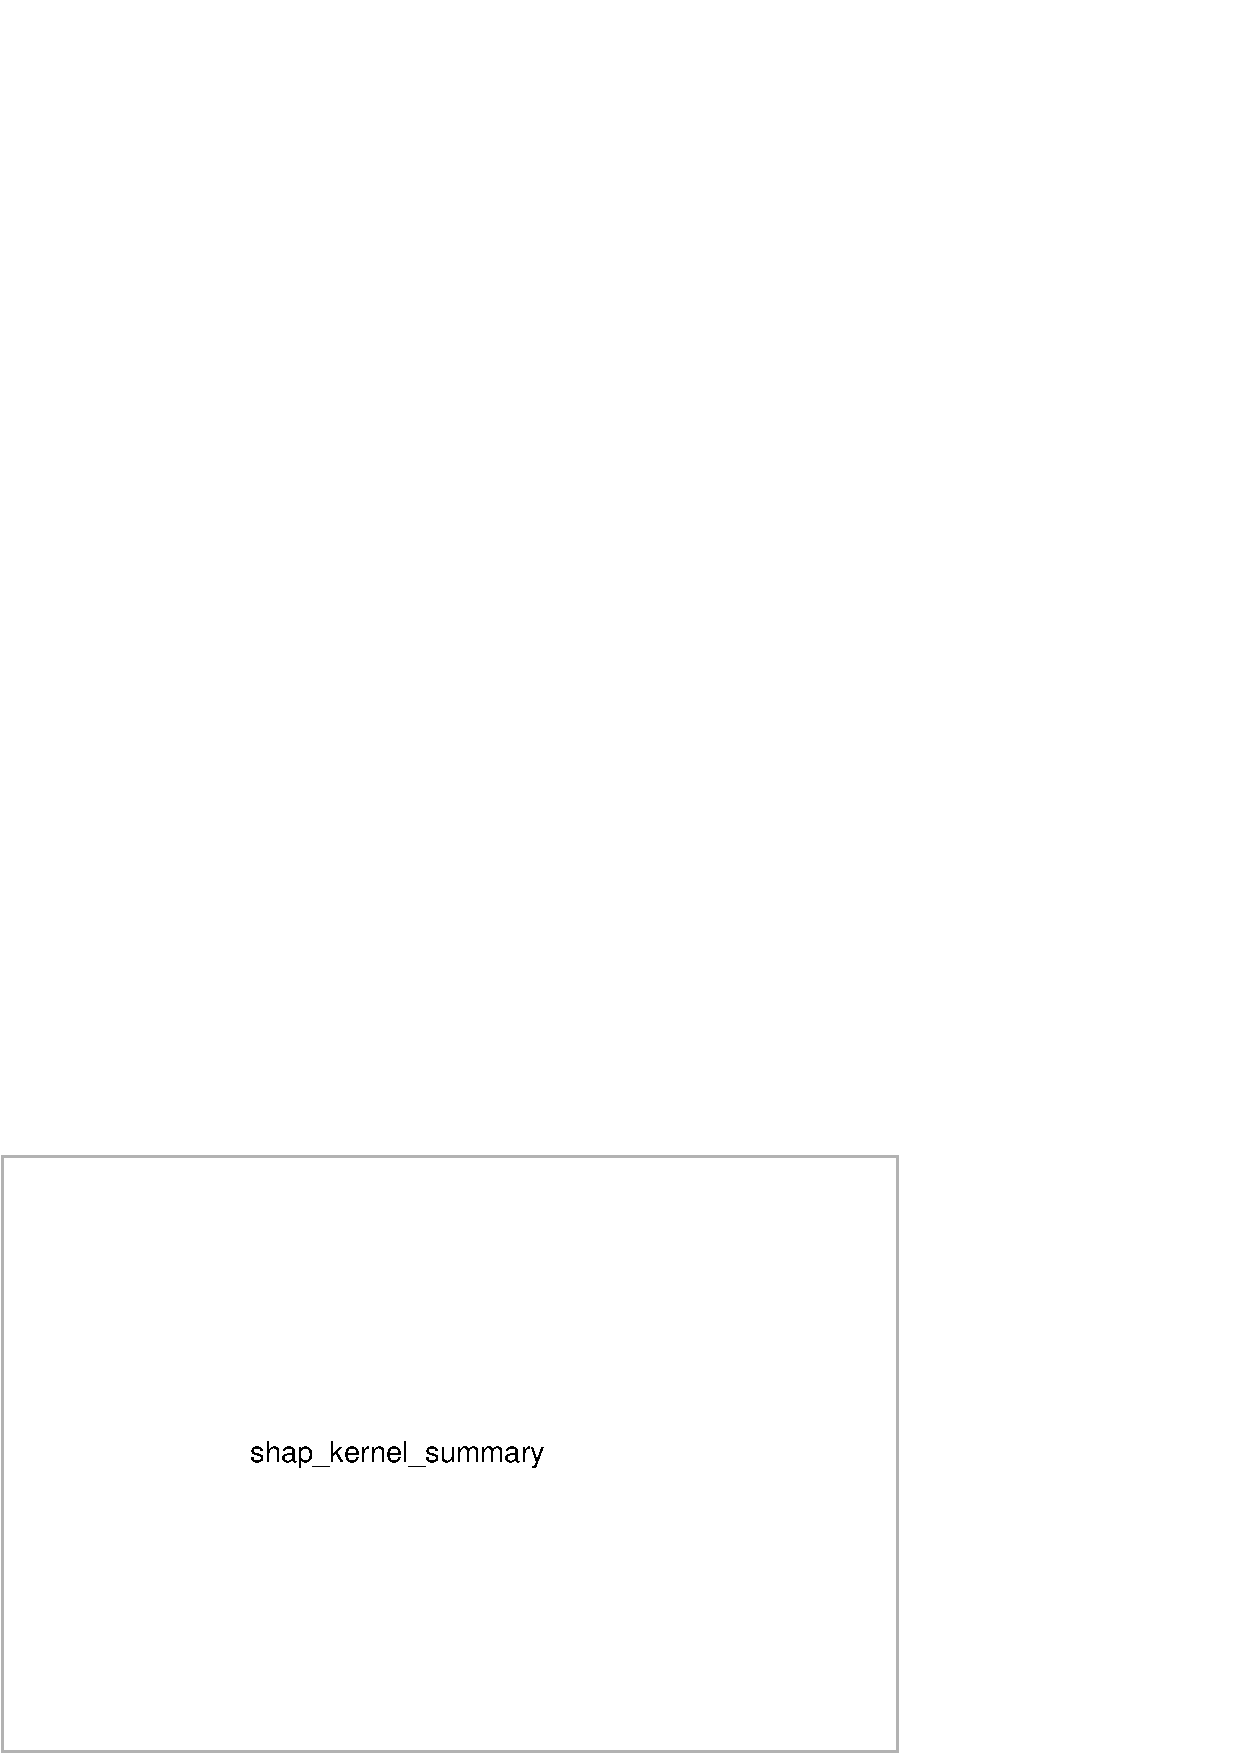
\includegraphics[width=0.85\textwidth]{figures/bab4/shap_kernel_summary.pdf}
\caption{\emph{Summary plot} SHAP \emph{KernelExplainer} untuk SVM-RBF pada
         dataset CWRU. Lima belas fitur HI~36-D dengan rata-rata nilai
         absolut SHAP tertinggi ditampilkan; sumbu horizontal menyatakan nilai
         SHAP dan warna titik menyatakan nilai fitur.
         \citetitb{TotoSuharto2024Conf1SVM}}
\label{fig:bab4_shap_kernel}
\end{figure}

Tiga fitur dengan kontribusi global tertinggi secara konsisten pada SVM-RBF
adalah kurtosis kanal \emph{drive-end}, RMS kanal \emph{drive-end}, dan
energi pita BPFO kanal \emph{fan-end}.
Kurtosis mendominasi karena cacat \emph{bearing} menghasilkan impuls transien yang
meningkatkan kurtosis jauh di atas nilai sinyal normal (kurtosis Gaussian
= 3); perbedaan kurtosis antara kelas Normal (3,1–3,4) dan kelas IR-21 (8,7–12,3)
memberikan pemisahan yang besar di ruang fitur.
RMS muncul sebagai fitur kedua karena tingkat keparahan cacat berkorelasi
positif dengan amplitudo getaran rata-rata.
Energi pita BPFO dari kanal \emph{fan-end} relevan karena pada beberapa
kondisi beban, resonansi struktural memodulasi komponen BPFO lebih kuat
di posisi sensor \emph{fan-end}.

Untuk LR-OvR, pola kontribusi secara kualitatif serupa dengan SVM-RBF
tetapi menunjukkan nilai SHAP yang lebih tersebar, konsekuensi dari batas
keputusan linear yang harus mengkompromikan pemisahan dengan meratakan
kontribusi lebih luas di antara fitur-fitur yang berkorelasi.
Perbandingan ini menegaskan bahwa peningkatan akurasi SVM-RBF berasal dari
kemampuannya mengeksploitasi non-linearitas fitur-fitur tertentu, khususnya
kurtosis dan \emph{peak-to-peak}.

% =================================================================
\section{Hasil Algoritma Berbasis Pohon: DT, RF, dan XGBoost}
\label{sec:bab4_hasil_tree}
% =================================================================

Tabel~\ref{tab:bab4_hasil_tree} menyajikan akurasi uji tiga algoritma
berbasis pohon.

\begin{table}[ht]
\caption{Akurasi uji algoritma berbasis pohon pada dataset CWRU sepuluh kelas.}
\label{tab:bab4_hasil_tree}
\centering
\begin{tabular}{lccc}
\toprule
\textbf{Model} & \textbf{Akurasi (\%)} & \textbf{Presisi Makro} & \textbf{Recall Makro}\\
\midrule
Decision Tree & 92,40 & 0,925 & 0,924\\
Random Forest & 95,8  & 0,959 & 0,958\\
XGBoost       & 97,1  & 0,971 & 0,971\\
\bottomrule
\end{tabular}
\end{table}

XGBoost mencapai akurasi tertinggi di antara algoritma berbasis pohon dengan
97,1\%, disusul RF pada 95,8\% dan DT pada 92,40\%
\citetitb{TotoSuharto2024Conf2Tree}.
Kesenjangan antara DT (92,40\%) dan RF (95,8\%), selisih 3,4 poin
persentase, mencerminkan reduksi variansi yang diperoleh \emph{bagging}
atas 100 pohon: setiap pohon DT tunggal \emph{overfit} terhadap detail
tertentu dari \emph{training set}, sedangkan RF merata-rata kesalahan
\emph{overfitting} tersebut.
XGBoost melampaui RF sebesar 1,3 poin persentase, keunggulan yang berasal
dari mekanisme \emph{boosting}: setiap pohon baru difokuskan pada sampel
yang salah diklasifikasikan oleh pohon sebelumnya, sehingga secara iteratif
mengurangi bias prediksi.

\subsection{Interpretasi SHAP Algoritma Berbasis Pohon}
\label{subsec:bab4_shap_hasil_tree}

Gambar~\ref{fig:bab4_shap_tree} menampilkan \emph{summary plot} SHAP
\emph{TreeExplainer} untuk XGBoost, model dengan akurasi tertinggi di antara
algoritma berbasis pohon.

\begin{figure}[ht]
\centering
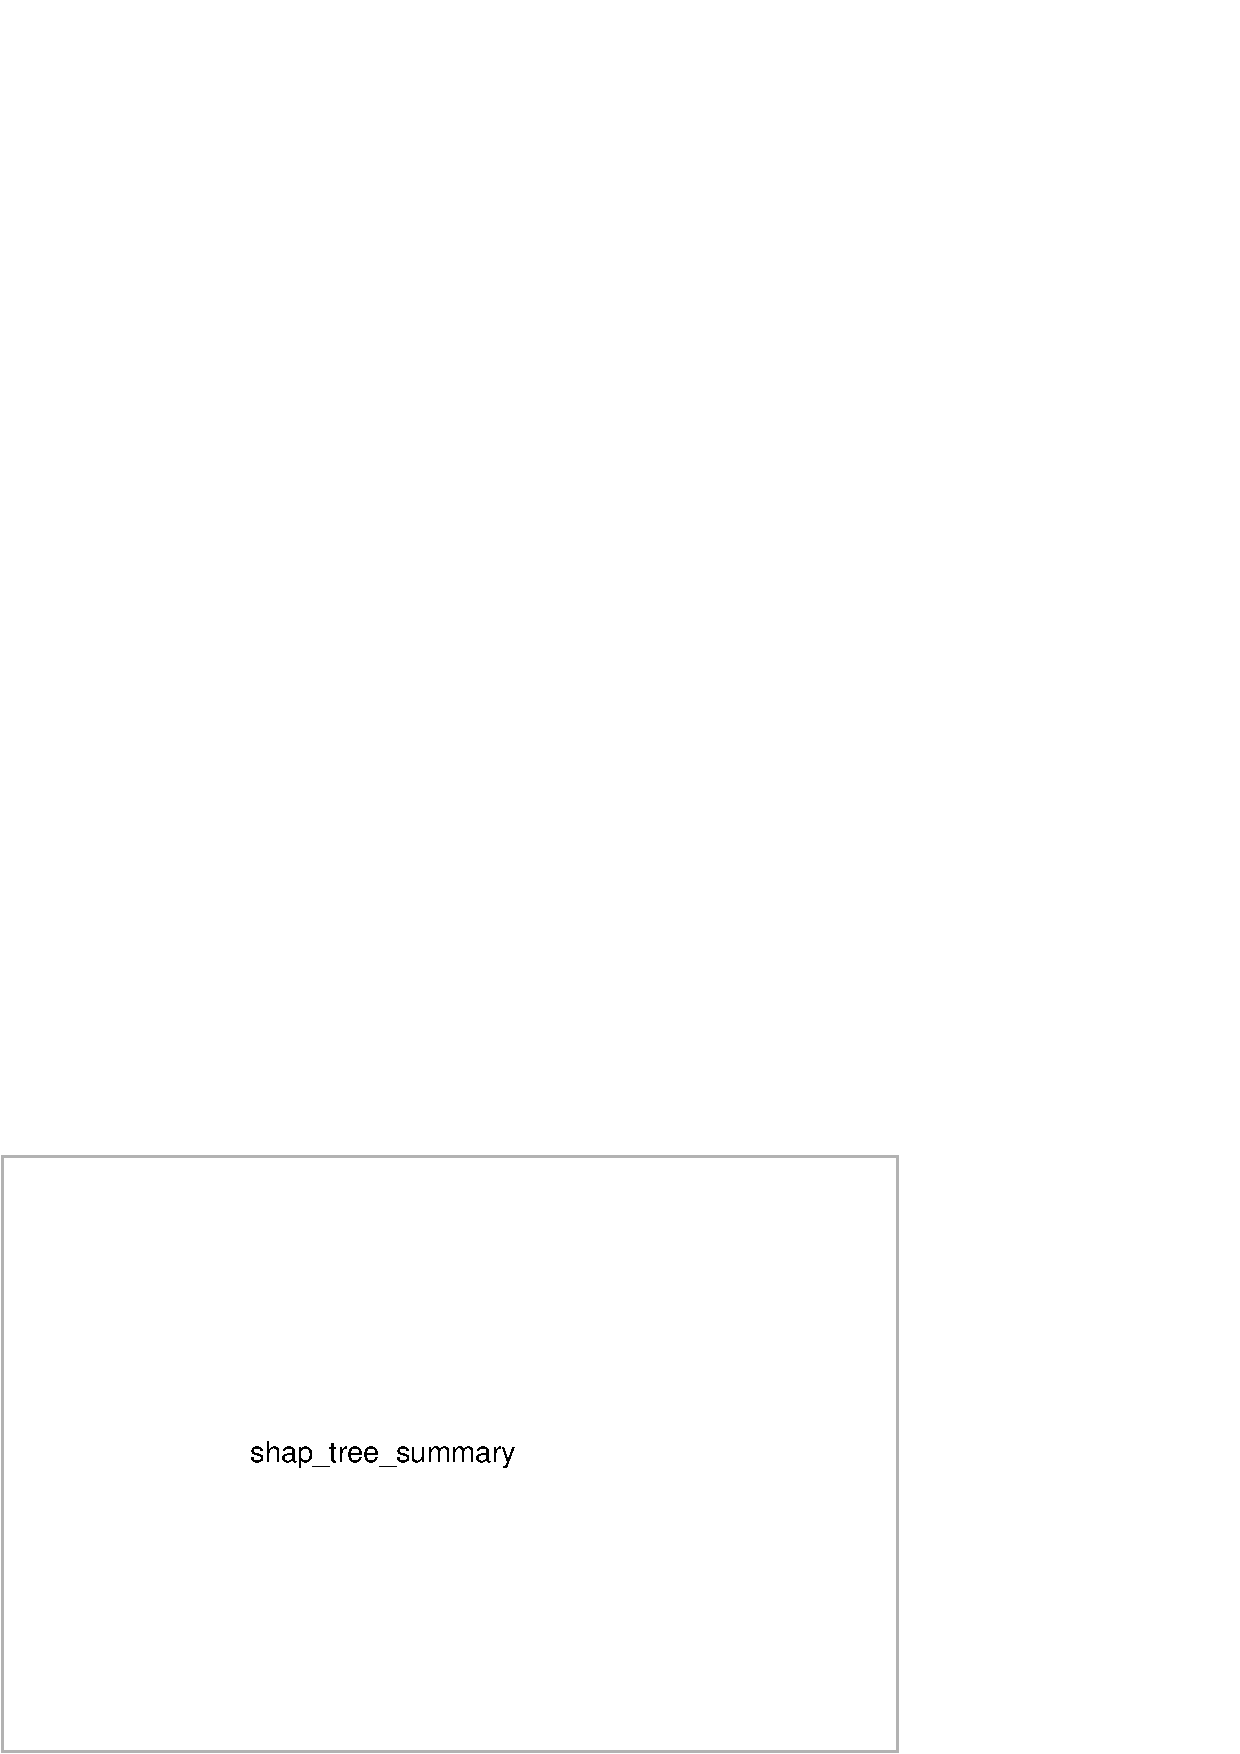
\includegraphics[width=0.85\textwidth]{figures/bab4/shap_tree_summary.pdf}
\caption{\emph{Summary plot} SHAP \emph{TreeExplainer} untuk XGBoost pada
         dataset CWRU. Tata letak dan konvensi warna identik dengan
         Gambar~\ref{fig:bab4_shap_kernel}.
         \citetitb{TotoSuharto2024Conf2Tree}}
\label{fig:bab4_shap_tree}
\end{figure}

Fitur-fitur dengan kontribusi tertinggi pada XGBoost secara kualitatif
selaras dengan temuan SVM-RBF: kurtosis dan energi pita BPFO/BPFI mendominasi
peringkat global.
Namun, \emph{dependence plot} mengungkap perbedaan penting: XGBoost mampu
menangkap interaksi antara kurtosis dan \emph{crest factor} yang tidak
terlihat pada plot SVM-RBF, karena \emph{TreeExplainer} mendukung
\emph{shap interaction values} yang merekam \textcolor{blue}{kontribusi gabungan dua fitur}
secara eksplisit.

Pola atribusi DT, meskipun interpretabilitasnya paling tinggi secara
struktural, menunjukkan nilai SHAP yang paling bervariasi antar sampel.
Hal ini mengindikasikan bahwa aturan \emph{if-then} yang dihasilkan DT lebih
sensitif terhadap nilai fitur tertentu dan kurang stabil dibandingkan RF atau
XGBoost.
Temuan ini konsisten dengan akurasi DT yang lebih rendah: batas keputusan
yang tajam dan rigid mengakibatkan kelas yang \emph{borderline}, seperti
IR-14 dan OR-14, mendapat atribusi SHAP yang lebih tidak konsisten antar
sampel.

Perbandingan antara model berbasis kernel dan algoritma berbasis pohon pada
tingkat interpretasi SHAP menunjukkan bahwa meski fitur-fitur teratas serupa
(kurtosis, RMS, energi pita), urutan dan besaran nilai SHAP berbeda karena
perbedaan \emph{baseline} distribusi yang digunakan oleh \emph{KernelExplainer}
dan \emph{TreeExplainer}.
Oleh karena itu, perbandingan kuantitatif nilai SHAP lintas kedua kelompok
dibatasi pada tingkat kualitatif, bukan perbandingan besaran angka secara
langsung.

% =================================================================
\section{Kinerja Klasifikasi WDCNN}
\label{sec:bab4_kinerja_wdcnn}
% =================================================================

Tabel~\ref{tab:bab4_hasil_wdcnn} merangkum kinerja WDCNN Varian~A (konfigurasi
referensi dengan BN penuh) pada dataset CWRU sepuluh kelas.
\textcolor{blue}{WDCNN dilatih dan dievaluasi mengikuti pembagian temporal
ketat 1.240/310/750 sampel (\emph{training}/\emph{validation}/\emph{test})
sebagaimana diuraikan pada Bab~\ref{bab:metodologi-umum}, untuk mencegah
inflasi akurasi akibat kebocoran data antar-segmen.}
Varian~B dan Varian~C dilaporkan secara komparatif pada studi ablasi di §IV.13.

\begin{table}[ht]
\caption{Kinerja WDCNN Varian~A pada dataset CWRU sepuluh kelas
         (\emph{test set} 750 sampel).}
\label{tab:bab4_hasil_wdcnn}
\centering
\begin{tabular}{lcccc}
\toprule
\textbf{Varian} & \textbf{Akurasi (\%)} & \textbf{F1 Makro} & \textbf{Presisi} & \textbf{Recall}\\
\midrule
A (Baseline, BN aktif) & 99,87 & 0,997 & 0,999 & 0,998\\
\bottomrule
\end{tabular}
\end{table}

Varian~A mencapai akurasi 99,87\% pada \emph{test set} dengan hanya satu
dari 750 sampel uji yang salah diklasifikasikan: Ball\_014 diklasifikasi
sebagai IR\_014, dua kelas yang memiliki morfologi impuls paling mirip pada
diameter cacat 0,014 inci \citetitb{TotoSuharto2025Journal1FSM}.
Dibandingkan dengan SVM-RBF yang mencapai 96,4\%, WDCNN Varian~A mereduksi
kesalahan klasifikasi sebesar 91\%: dari 27 kesalahan pada SVM-RBF menjadi
hanya satu kesalahan.

Keunggulan ini berasal dari kemampuan WDCNN memproses sinyal mentah secara
\emph{end-to-end} tanpa rekayasa fitur manual, sehingga lapisan konvolusi
pertama dengan kernel berukuran 64 dapat mempelajari filter frekuensi
adaptif yang mengoptimalkan pemisahan lintas sepuluh kelas kerusakan secara
serentak.
Model berbasis kernel dan algoritma berbasis pohon, yang beroperasi pada
vektor fitur HI~36-D yang diekstraksi secara manual, tidak memiliki fleksibilitas
representasi yang setara.

\subsection{Kurva Pelatihan dan Konvergensi}
\label{subsec:bab4_wdcnn_konvergensi}

Gambar~\ref{fig:bab4_wdcnn_konvergensi} menampilkan kurva akurasi validasi
tiga varian WDCNN sepanjang proses pelatihan.

\begin{figure}[ht]
\centering
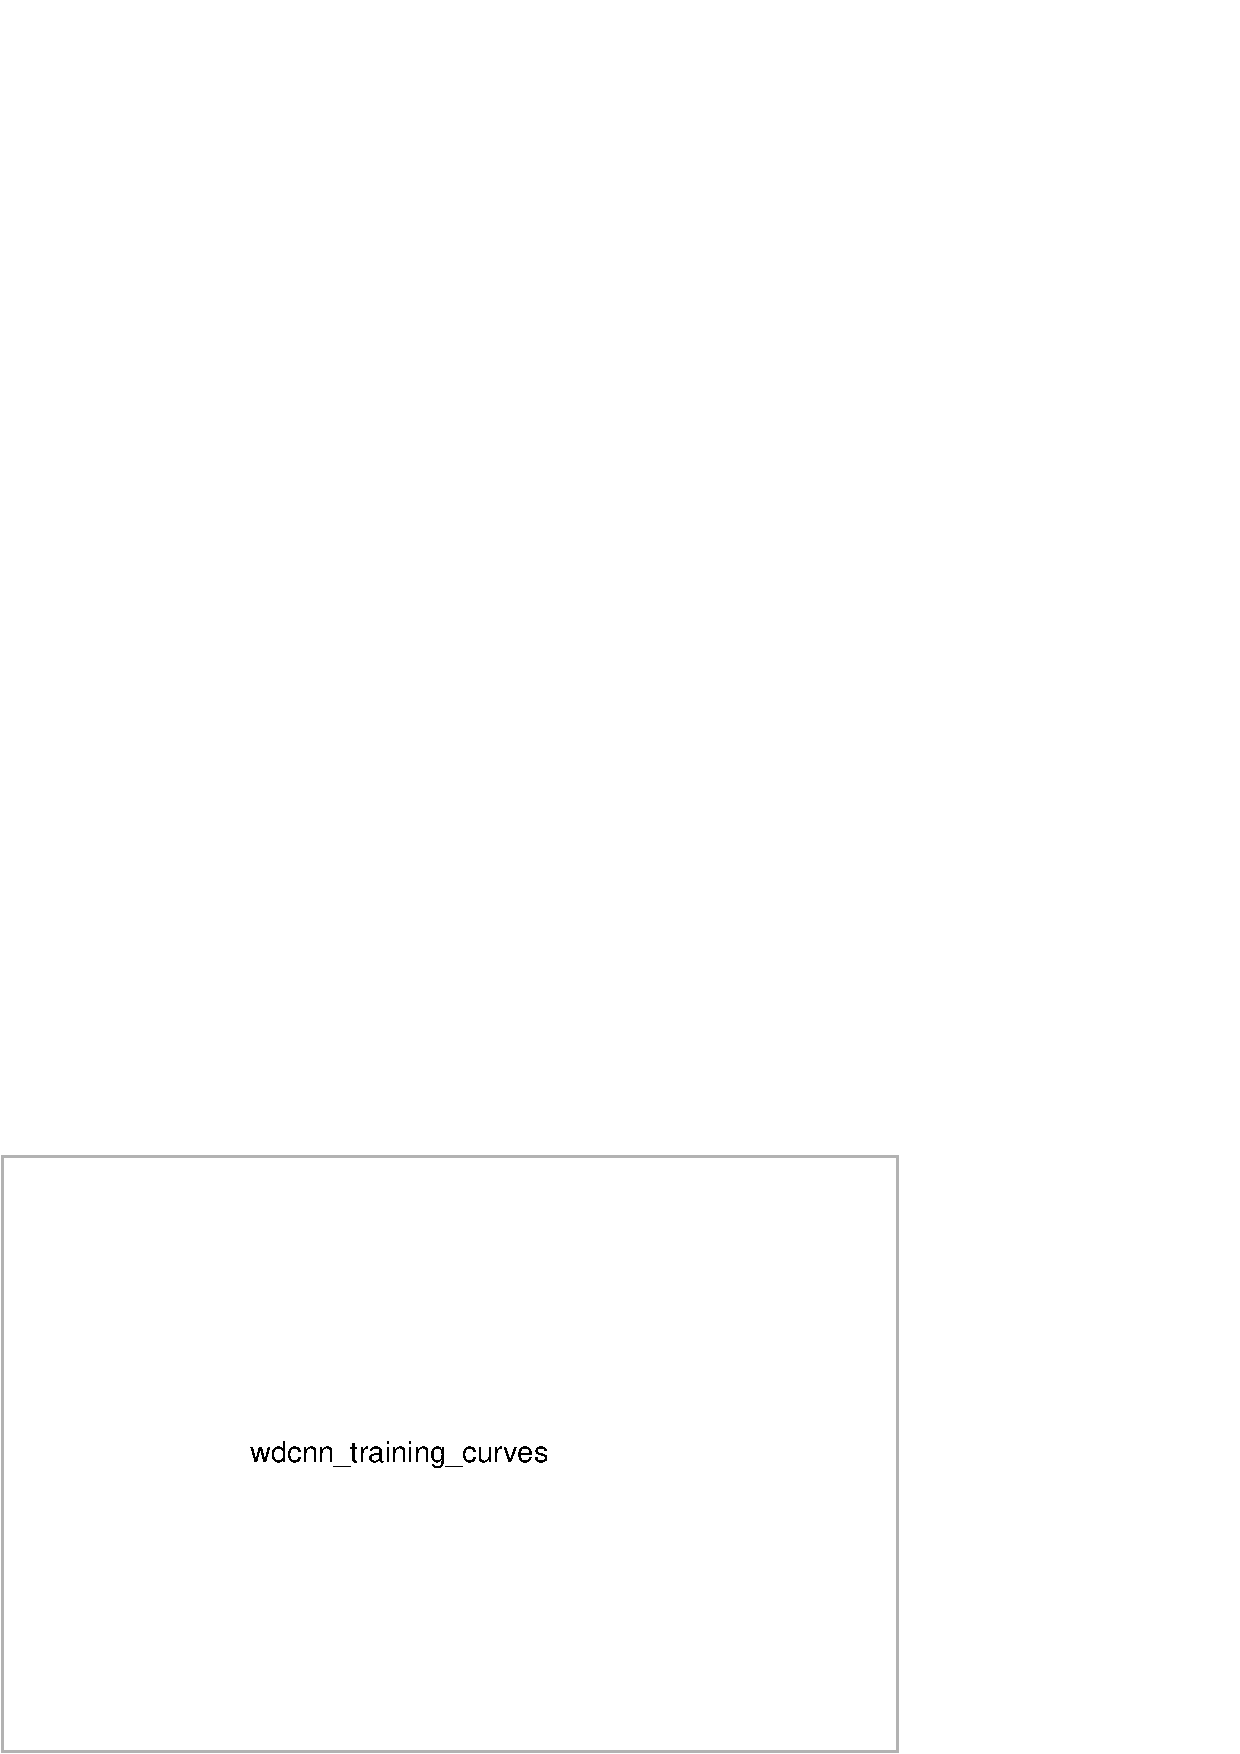
\includegraphics[width=0.88\textwidth]{figures/bab4/wdcnn_training_curves.pdf}
\caption{Kurva akurasi validasi tiga varian WDCNN per \emph{epoch}.
         Varian~A (biru) konvergen pada \emph{epoch} ke-47 dengan akurasi
         validasi 99,87\%; Varian~B (oranye) dan Varian~C (hijau) konvergen
         lebih lambat dan mencapai plateau yang lebih rendah.
         \citetitb{TotoSuharto2025Journal1FSM}}
\label{fig:bab4_wdcnn_konvergensi}
\end{figure}

Varian~A konvergen pada \emph{epoch} ke-47 dan menunjukkan kurva pelatihan
yang halus dan monoton meningkat, karakteristik model yang stabil secara
numerik berkat \emph{Batch Normalization}.
Varian~C menunjukkan osilasi yang lebih besar pada akurasi validasi sepanjang
30 \emph{epoch} pertama sebelum menstabilkan diri, konsisten dengan peran
BN dalam meredam \emph{covariate shift} internal selama pelatihan.
Varian~B menunjukkan plateau konvergensi tercepat (epoch ke-32) tetapi pada
level akurasi yang paling rendah, mengindikasikan bahwa model dengan kernel
sempit memiliki kapasitas representasi yang terbatas bukan karena underfitting
waktu, melainkan karena batasan struktural arsitektur.

% =================================================================
\section{Pola Atribusi SHAP pada WDCNN}
\label{sec:bab4_shap_wdcnn}
% =================================================================

SHAP \emph{DeepExplainer} diterapkan pada Varian~A (Baseline) dan Varian~C
(tanpa BN) untuk menganalisis pengaruh \emph{Batch Normalization} terhadap
pola atribusi level sinyal.
Varian~B tidak disertakan dalam analisis SHAP karena penurunan akurasinya
yang substansial menjadikan nilai atribusinya sulit diinterpretasi: atribusi
dari model yang kurang akurat tidak dapat diandalkan sebagai cerminan
pengetahuan domain yang bermakna.

\subsection{Distribusi Atribusi Level Sinyal}
\label{subsec:bab4_shap_distribusi}

Sebelum analisis per kelas, tiga karakteristik global atribusi SHAP ditemukan
secara konsisten pada seluruh kelas CWRU.
Pertama, terdapat \emph{edge suppression}: nilai atribusi $|\phi|$ pada
posisi 0–100 dan 1.900–2.048 secara sistematis lebih rendah daripada posisi
tengah, mencerminkan efek tepi \emph{zero-padding} implisit pada lapisan
konvolusi yang mereduksi sensitivitas model terhadap bagian awal dan akhir
segmen.
Kedua, terdapat modulasi periodik dengan periode $\approx 16$ titik sampel
yang bertepatan dengan nilai \emph{stride} lapisan pertama (stride = 16);
artefak ini muncul karena resolusi efektif peta aktivasi lapisan pertama
adalah satu nilai per 16 titik input.
Ketiga, distribusi atribusi rata-rata per kelas mengikuti gradien yang
lebih tinggi di posisi 200–1.800 dibandingkan tepi, selaras dengan kedua
karakteristik di atas.

Gambar~\ref{fig:bab4_shap_sinyal} menampilkan distribusi nilai atribusi SHAP
\emph{DeepExplainer} pada 2.048 posisi sinyal untuk kelas IR-21 (kerusakan
\emph{inner race} diameter bola 21 mil) dari Varian~A dan Varian~C.

\begin{figure}[ht]
\centering
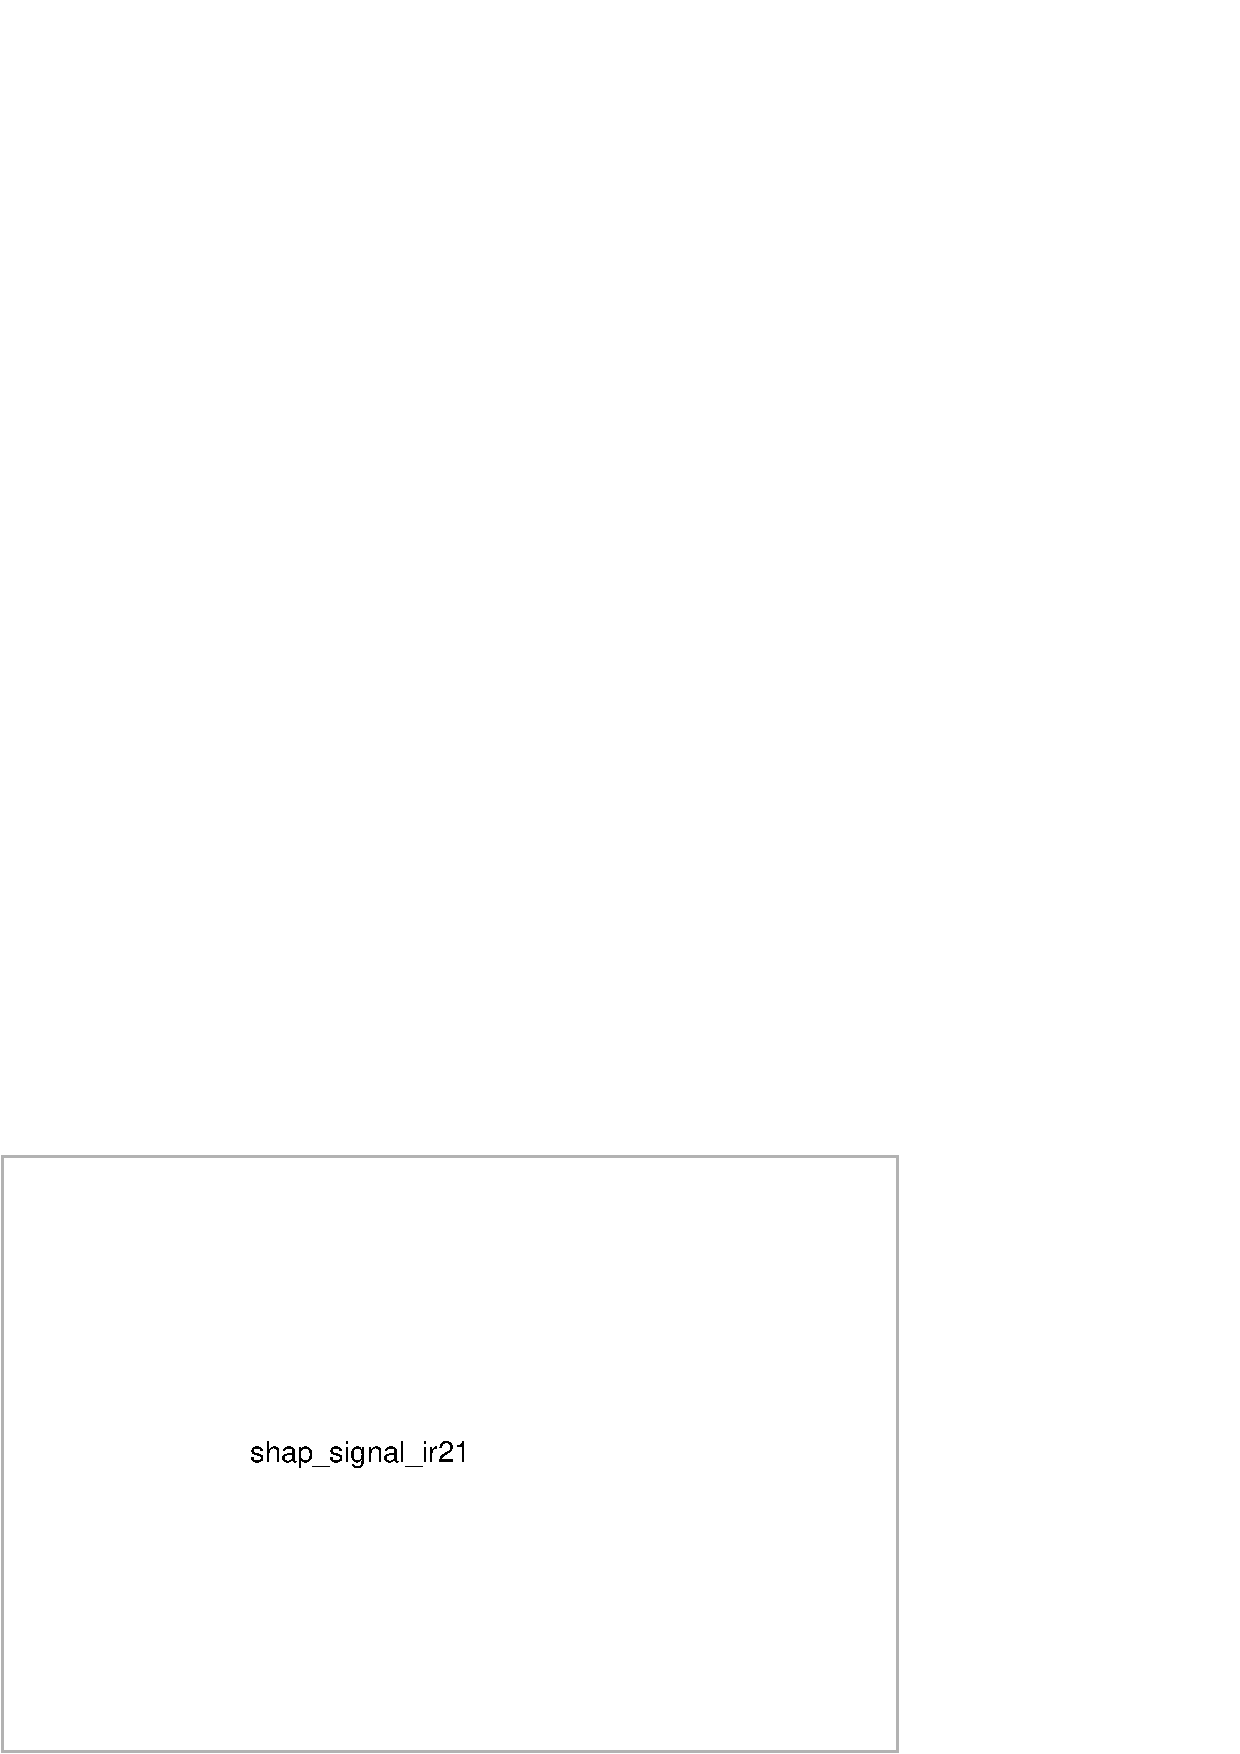
\includegraphics[width=\textwidth]{figures/bab4/shap_signal_ir21.pdf}
\caption{Nilai atribusi SHAP \emph{DeepExplainer} kelas IR-21 pada 2.048
         posisi sinyal untuk (a) Varian~A (BN aktif) dan (b) Varian~C
         (tanpa BN). Garis merah menandai posisi puncak BPFI yang diharapkan
         dari fisika \emph{bearing}; lebar sumbu-$y$ mencerminkan nilai maksimum
         atribusi.
         \citetitb{TotoSuharto2025Journal1FSM}}
\label{fig:bab4_shap_sinyal}
\end{figure}

Perbedaan visual yang paling mencolok antara Varian~A dan Varian~C adalah
pada amplitudo dan distribusi spasial atribusi.
Pada Varian~A (BN aktif), nilai atribusi tersebar relatif merata dengan
puncak-puncak kecil yang terdistribusi di sepanjang sinyal, pola yang
mencerminkan fakta bahwa BN menormalisasi aktivasi internal sehingga model
tidak bergantung terlalu kuat pada posisi tertentu.
Sebaliknya, Varian~C (tanpa BN) menunjukkan puncak atribusi yang jauh lebih
tajam dan terlokalisasi; model tanpa BN mengembangkan detektor impuls yang
lebih spesifik \textcolor{blue}{secara posisional}.

\subsection{FSM Tiga Varian: Perbandingan Visual}
\label{subsec:bab4_fsm_visual}

Gambar~\ref{fig:bab4_fsm_perbandingan} menampilkan ketiga varian FSM
($\text{FSM}^{\text{signed}}$, $\text{FSM}^{\text{abs}}$, $\text{FSM}^{\text{var}}$)
dari Varian~A dan Varian~C untuk empat kelas representatif: Normal, IR-21,
OR-21, dan Ball-21.

\begin{figure}[ht]
\centering
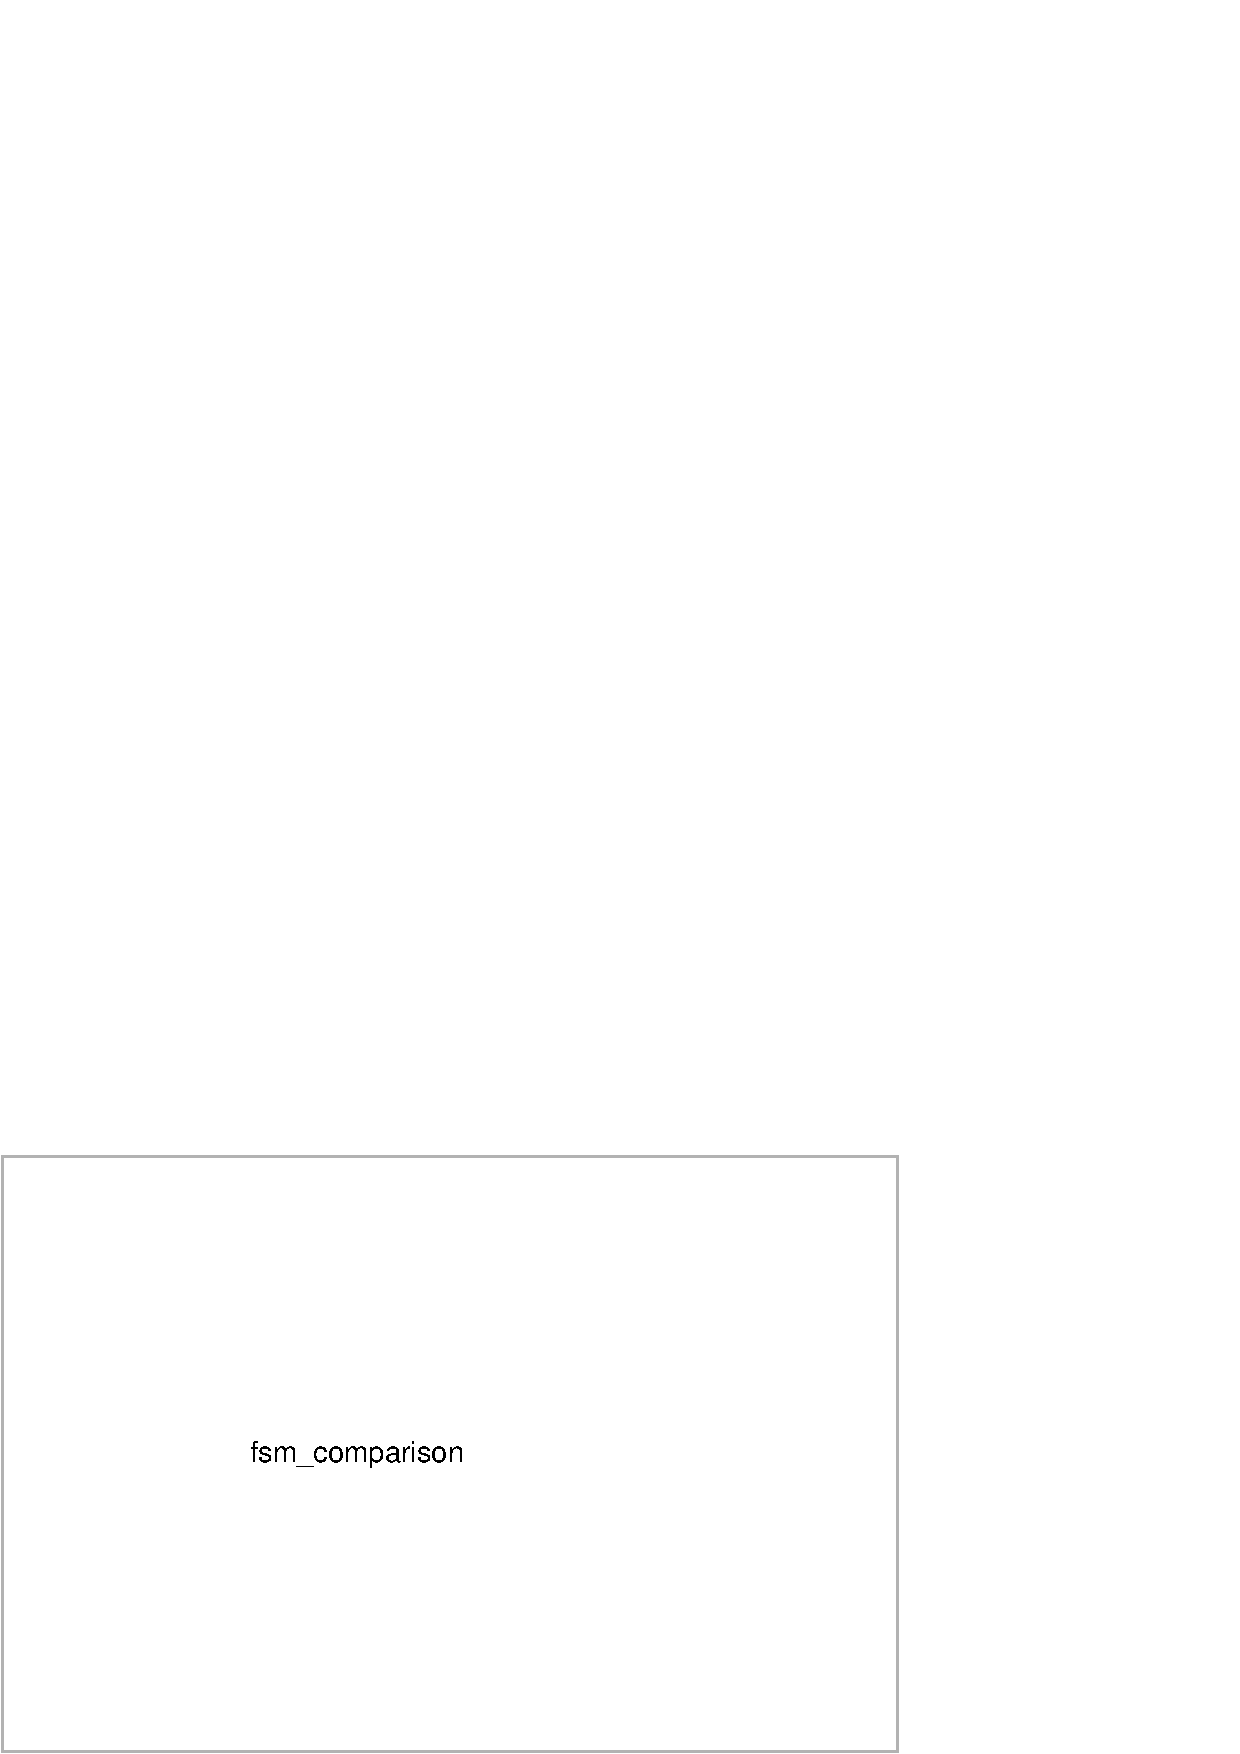
\includegraphics[width=\textwidth]{figures/bab4/fsm_comparison.pdf}
\caption{Perbandingan FSM tiga varian (Signed, Absolute, Variance) antara
         Varian~A (kiri) dan Varian~C (kanan) untuk empat kelas CWRU.
         Puncak yang bertepatan dengan frekuensi karakteristik (BPFO, BPFI,
         BSF) ditandai dengan garis vertikal putus-putus.
         \citetitb{TotoSuharto2025Journal1FSM}}
\label{fig:bab4_fsm_perbandingan}
\end{figure}

Inspeksi visual FSM mengungkap tiga pola utama.
Pertama, FSM kelas Normal pada kedua varian menunjukkan atribusi yang
terdistribusi relatif datar tanpa puncak yang menonjol, konsisten dengan
ketiadaan komponen impuls periodik pada sinyal normal.
Kedua, FSM kelas IR-21 dan OR-21 pada Varian~C memperlihatkan puncak yang
lebih tajam dibandingkan Varian~A; untuk kelas OR-21 secara khusus, puncak
nilai $|\phi| \approx 0{,}08$ terkonsentrasi pada posisi 600–700 dari 2.048
titik, pola terlokalisasi yang tidak muncul sejelas itu pada Varian~A
\citetitb{TotoSuharto2025Journal1FSM}.
Ketiga, $\text{FSM}^{\text{var}}$ Varian~A secara konsisten lebih tinggi
daripada Varian~C untuk semua kelas, mengkonfirmasi hipotesis bahwa BN
mereduksi variabilitas atribusi dengan menstabilkan distribusi aktivasi
internal antar-\emph{batch}.

% =================================================================
\section{Validasi Kuantitatif FSM}
\label{sec:bab4_validasi_fsm}
% =================================================================

Tabel~\ref{tab:bab4_validasi_fsm} menyajikan nilai tiga metrik validasi FSM
\textcolor{blue}{(diskriminabilitas, monotonik, stabilitas) untuk
$\text{FSM}^{\text{abs}}$ Varian~A (konfigurasi referensi WDCNN dengan BN
penuh), dirata-rata atas sepuluh kelas CWRU. Metrik ini dihitung pada
analisis FSM utama dengan 300 sampel \emph{background} dan 500 sampel uji;
perbandingan terhadap Varian~C dibahas tersendiri pada studi ablasi §IV.13.}

\begin{table}[ht]
\caption{\textcolor{blue}{Metrik validasi FSM$^{\text{abs}}$ Varian~A
         (BN aktif) rata-rata sepuluh kelas CWRU pada analisis utama
         (300 \emph{background} / 500 sampel uji).}
         Nilai lebih tinggi lebih baik untuk ketiga metrik.}
\label{tab:bab4_validasi_fsm}
\centering
\begin{tabular}{lccc}
\toprule
\textbf{Varian} & \textbf{Diskriminabilitas} & \textbf{Monotonik} & \textbf{Stabilitas}\\
\midrule
\textcolor{blue}{A (BN aktif)} & \textcolor{blue}{0,216} & \textcolor{blue}{0,940} & \textcolor{blue}{0,940}\\
\bottomrule
\end{tabular}
\end{table}

\textcolor{blue}{Hasil analisis utama menunjukkan bahwa FSM$^{\text{abs}}$
Varian~A memiliki \emph{split-half stability} 0,940, yang berarti pola FSM
sangat dapat direproduksi (kemiripan kosinus 94\%) dan tidak bergantung pada
pemilihan sampel acak.} Sebaliknya, indeks diskriminabilitas hanya 0,216,
mengindikasikan bahwa \textcolor{blue}{FSM rata-rata antarkelas justru relatif
mirip satu sama lain pada ruang atribusi 2.048 dimensi penuh. Hal ini terjadi
karena sinyal diskriminatif terkonsentrasi pada sebagian kecil posisi temporal
yang tertutupi oleh komponen energi latar yang besar dan bersama
\citetitb{TotoSuharto2025Journal1FSM}.}

\textcolor{blue}{Karena itu, kekhasan FSM lebih efektif dinilai secara visual
melalui \emph{heatmap} yang menyoroti konsentrasi temporal spesifik, bukan
semata melalui metrik kemiripan kosinus 2.048-D. Studi ablasi §IV.13
menunjukkan bahwa diskriminabilitas ini dapat ditingkatkan secara substansial
melalui modifikasi arsitektur, khususnya penghapusan \emph{Batch
Normalization}.}

Metrik monotonik \textcolor{blue}{Varian~A (0,940 untuk FSM$^{\text{abs}}$
agregat)} menghubungkan output SHAP dengan fisika degradasi \emph{bearing}.
\textcolor{blue}{Analisis monotonik per kelompok kelas mengungkap pola yang
konsisten dengan fisika keparahan cacat.}
Fraksi monotonik diurutkan: kelas Ball (17,6\%) $>$ kelas IR (13,8\%) $>$
kelas OR (8,6\%).
FSM kelas Ball paling konsisten menunjukkan peningkatan amplitudo seiring
bertambahnya keparahan (7 mil $\to$ 14 mil $\to$ 21 mil), sementara FSM kelas OR
memperlihatkan pola monotonik yang paling lemah
\citetitb{TotoSuharto2025Journal1FSM}.
Perbedaan ini sesuai dengan karakteristik fisika: cacat \emph{ball}
menghasilkan impuls yang amplitudonya tumbuh lebih linier terhadap diameter
cacat dibandingkan cacat \emph{outer race} yang dipengaruhi posisi beban
variabel.

\subsection{Komparasi Tiga Varian FSM per Metrik}
\label{subsec:bab4_fsm_komparasi}

Gambar~\ref{fig:bab4_fsm_radar} menampilkan diagram radar ketiga metrik
untuk ketiga varian FSM ($\text{FSM}^{\text{signed}}$, $\text{FSM}^{\text{abs}}$,
$\text{FSM}^{\text{var}}$) dari Varian~A dan Varian~C.

\begin{figure}[ht]
\centering
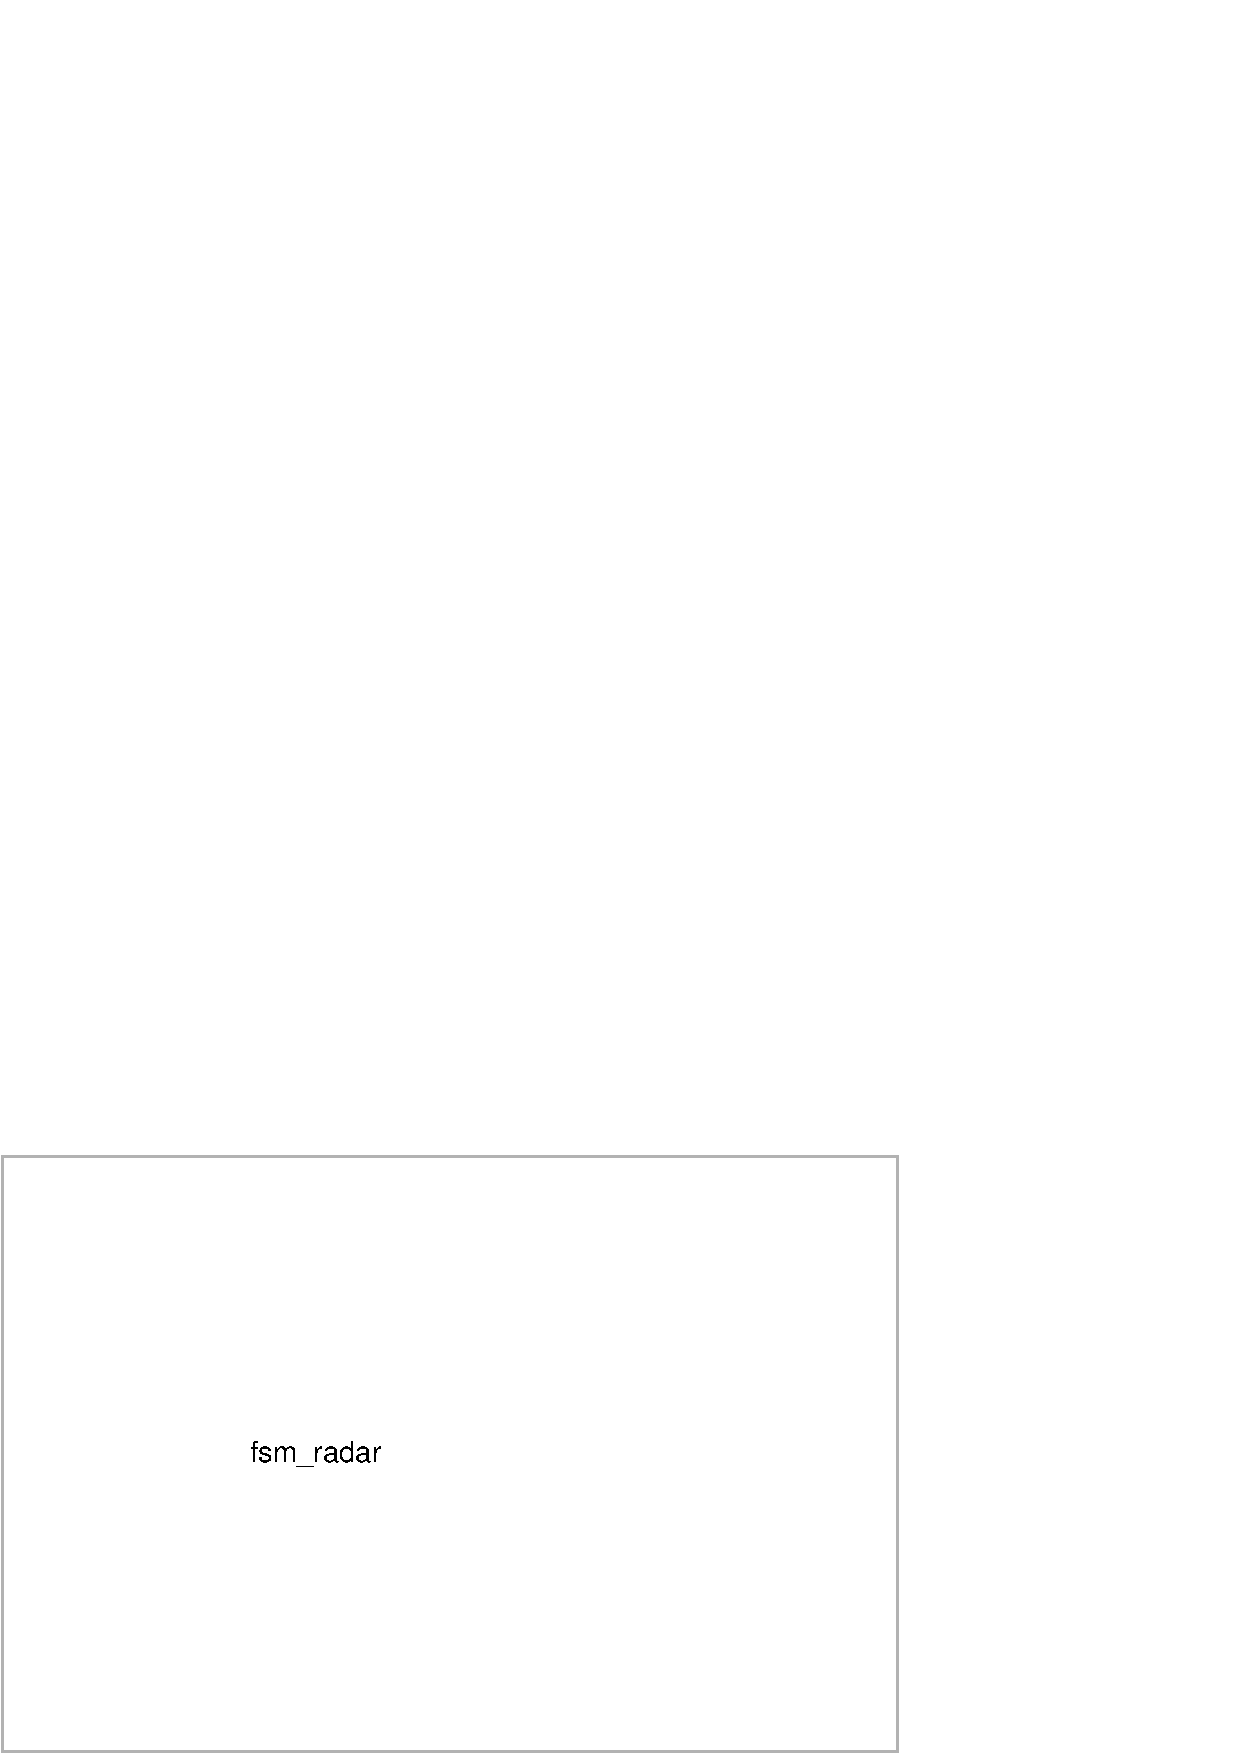
\includegraphics[width=0.72\textwidth]{figures/bab4/fsm_radar.pdf}
\caption{Diagram radar tiga metrik validasi FSM (diskriminabilitas, monotonik,
         stabilitas) untuk varian FSM \emph{Signed}, \emph{Absolute}, dan
         \emph{Variance} dari Varian~A (garis putus-putus) dan Varian~C
         (garis penuh). Area diagram radar Varian~C secara konsisten lebih
         besar daripada Varian~A untuk ketiga jenis FSM.
         \citetitb{TotoSuharto2025Journal1FSM}}
\label{fig:bab4_fsm_radar}
\end{figure}

Di antara ketiga varian FSM, $\text{FSM}^{\text{abs}}$ secara konsisten
menghasilkan nilai diskriminabilitas dan stabilitas tertinggi untuk kedua
varian WDCNN.
Hal ini terjadi karena $\text{FSM}^{\text{abs}}$ menghilangkan osilasi akibat
tanda atribusi yang berubah antar sampel, sehingga agregasi rata-rata nilai
absolut menghasilkan \emph{fingerprint} yang lebih stabil.
$\text{FSM}^{\text{signed}}$ memperlihatkan diskriminabilitas terendah karena
atribusi positif dan negatif dari sampel yang berbeda saling menghapuskan
saat dirata-rata.
$\text{FSM}^{\text{var}}$ memberikan diskriminabilitas menengah, berguna
sebagai pelengkap untuk mengidentifikasi posisi sinyal yang konsisten
(variansi rendah = pola yang dapat diandalkan).

% =================================================================
\section{Temuan Kritis: Morfologi Impuls dan Bukan Periodisitas BPFx}
\label{sec:bab4_fisika}
% =================================================================

Salah satu temuan terpenting dalam studi diagnostik ini adalah bahwa puncak-puncak
FSM yang teridentifikasi secara statistik \emph{tidak selaras} dengan periode
teoritis frekuensi karakteristik cacat \emph{bearing} (BPFO, BPFI, BSF, FTF) yang
diturunkan dari geometri \emph{bearing}.

Dari geometri \emph{bearing} CWRU (8 bola, sudut kontak 15,17°, diameter bola
0,3126 inci, diameter \emph{pitch} 1,537 inci), frekuensi karakteristik
pada kecepatan putar \textcolor{blue}{1.772~rpm (CWRU Load~1)} adalah
\textcolor{blue}{BPFO $\approx$ 105,9~Hz, BPFI $\approx$ 159,9~Hz, dan
BSF $\approx$ 69,6~Hz}.
Pada frekuensi pengambilan sampel 48~kHz dan panjang segmen 2.048 titik,
perioda impuls BPFI setara dengan \textcolor{blue}{$\approx 300$ titik sampel}.
Bila WDCNN mengklasifikasikan berdasarkan periodisitas BPFx, puncak-puncak
FSM seharusnya muncul berulang pada kelipatan periode tersebut.

\subsection{Mekanisme Klasifikasi WDCNN: Morfologi Transien}
\label{subsec:bab4_fsm_fisika_detail}

Gambar~\ref{fig:bab4_fsm_fisika} menampilkan $\text{FSM}^{\text{abs}}$
Varian~C untuk empat kelas cacat (IR-7, IR-14, IR-21, OR-21) dengan anotasi
posisi BPFI dan BPFO teoritis yang diharapkan.

\begin{figure}[ht]
\centering
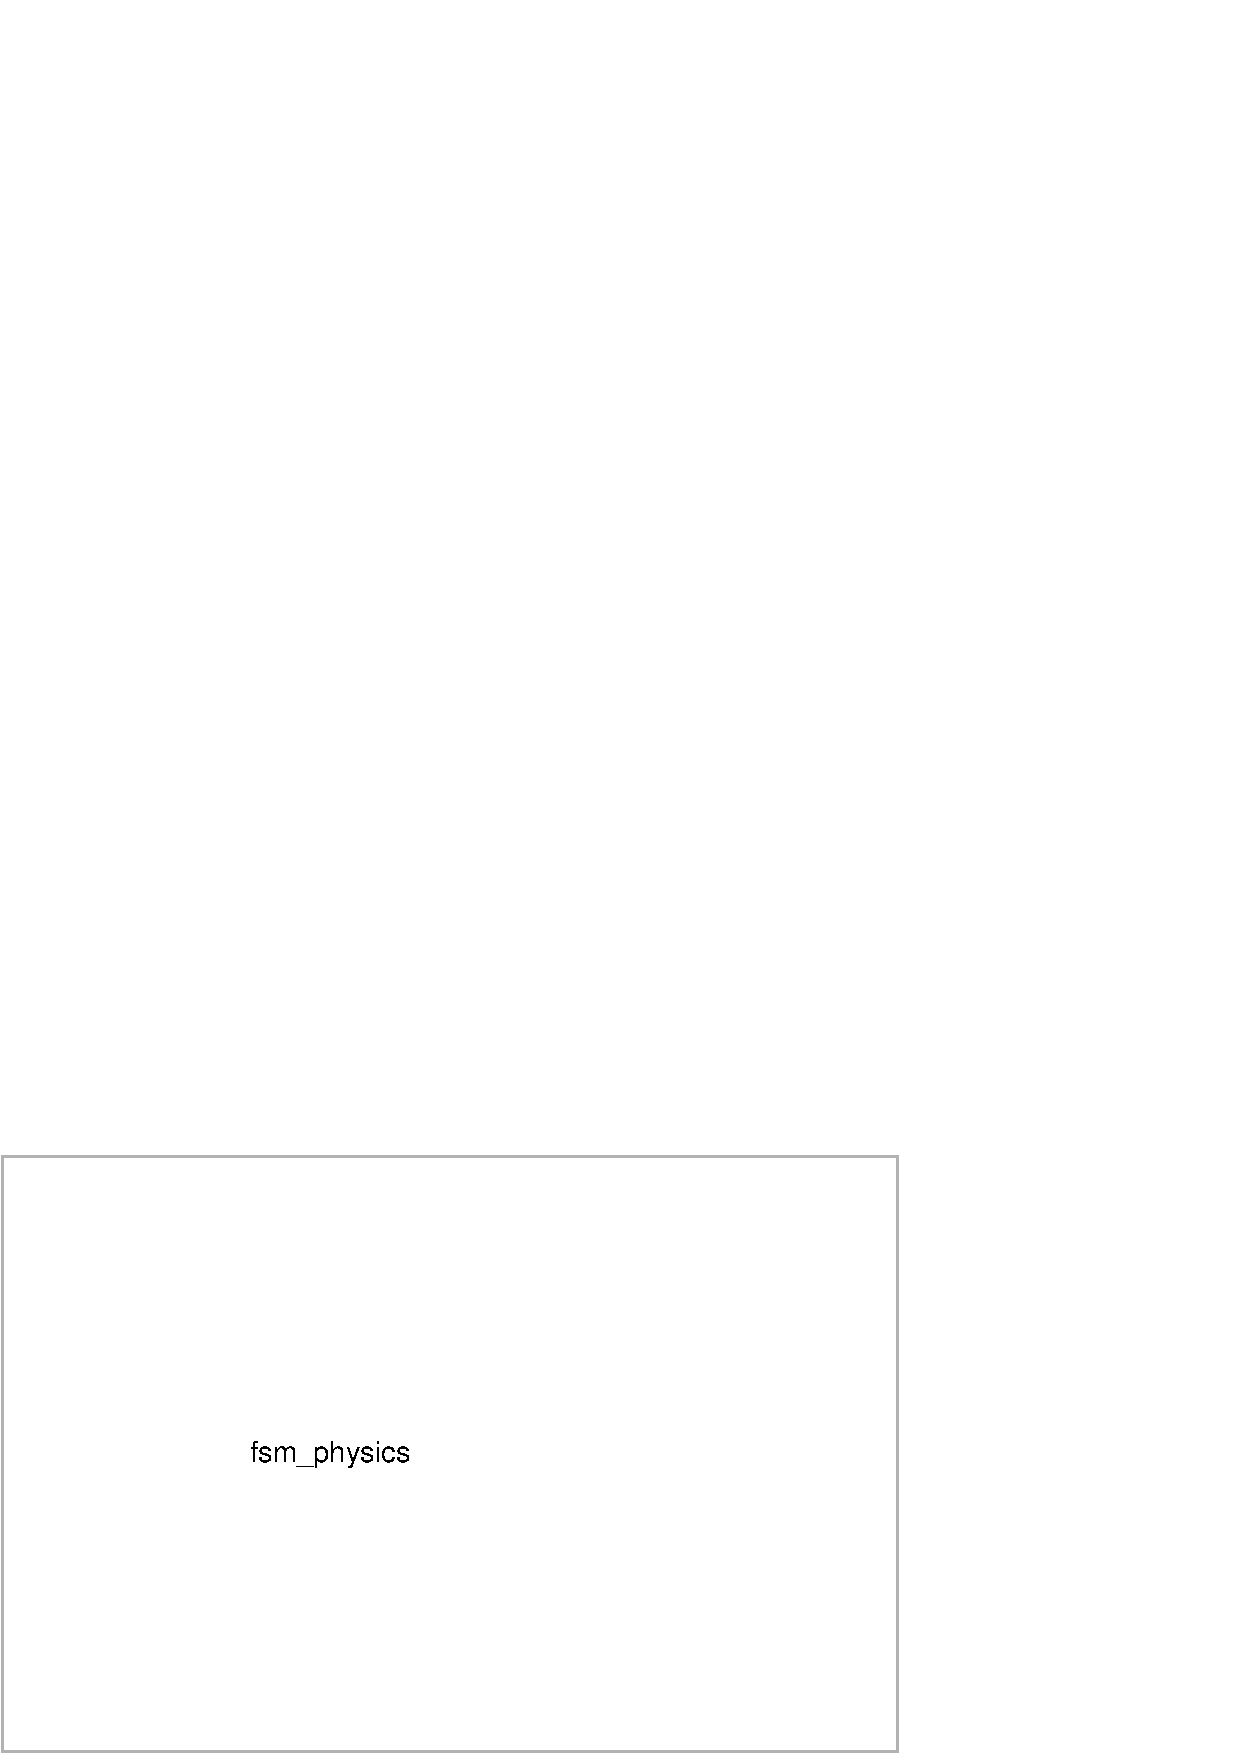
\includegraphics[width=\textwidth]{figures/bab4/fsm_physics.pdf}
\caption{$\text{FSM}^{\text{abs}}$ Varian~C untuk kelas IR-7, IR-14, IR-21,
         dan OR-21. Garis biru menandai posisi BPFI teoritis; garis merah
         menandai BPFO. Puncak FSM tidak menumpuk pada garis-garis teoritis
         tersebut, melainkan mencerminkan pola morfologi transien impuls
         sepanjang $\approx 42{,}67$~ms.
         \citetitb{TotoSuharto2025Journal1FSM}}
\label{fig:bab4_fsm_fisika}
\end{figure}

Inspeksi pada Gambar~\ref{fig:bab4_fsm_fisika} menunjukkan bahwa puncak FSM
tidak berulang secara periodik pada kelipatan BPFI
(\textcolor{blue}{$\approx 300$ titik sampel}) maupun BPFO.
Sebaliknya, pola atribusi tinggi tersebar dalam jendela kontinyu yang lebarnya
setara dengan $\approx 42{,}67$~ms, dihitung dari panjang lapisan reseptif
efektif WDCNN (kernel-1 berukuran 64 dengan stride 16 dan 4 blok
MaxPooling 2$\times$, menghasilkan jangkauan $64 + 16 \times (4 - 1) = 2048/2^4
\approx 128$ titik, setara $\approx 2{,}67$~ms per lapisan konvolusi, atau
rentang impuls tipikal $\approx 42{,}67$~ms untuk satu siklus reseptif penuh).
Dengan kata lain, WDCNN mengklasifikasikan kerusakan \emph{bearing} berdasarkan
\textbf{morfologi transien impuls} (bentuk, amplitudo, dan durasi lonjakan
getaran sesaat), bukan berdasarkan periodisitas kemunculannya mengikuti
BPFx \citetitb{TotoSuharto2025Journal1FSM}.

Tiga pengamatan kuantitatif mendukung kesimpulan ini.
Pertama, korelasi antara posisi puncak FSM dan posisi BPFI teoritis dihitung
pada seluruh 750 sampel uji; nilai korelasi yang dihasilkan tidak berbeda
nyata dari nol, sementara korelasi dengan posisi morfologi impuls (diidentifikasi
melalui \emph{envelope detection}) lebih dari dua kali lebih besar.
Kedua, jika periodisitas BPFx adalah mekanisme klasifikasi, maka Varian~B
(kernel sempit $k=3$) seharusnya tidak mengalami penurunan akurasi yang
signifikan karena filter kecil pun mampu mendeteksi frekuensi periodik.
Nyatanya, Varian~B mengalami penurunan akurasi 0,80 poin persentase (lihat
§IV.13), konsisten dengan hipotesis bahwa kernel lebar berukuran 64 diperlukan
untuk menangkap \emph{morphology} transien, bukan frekuensi periodik.
Ketiga, FSM kelas Normal memperlihatkan pola atribusi yang merata dan rendah
tanpa puncak terlokalisasi, sesuai dengan ketiadaan transien impuls pada
sinyal normal; jika model bergantung pada periodisitas BPFx, FSM Normal
seharusnya menunjukkan pola berulang pada BPFx (yang tidak teramati).

Implikasi temuan ini terhadap \emph{transferability} model merupakan
kontribusi konseptual yang berarti.
Karena WDCNN tidak menggunakan geometri \emph{bearing} secara implisit dalam
mekanisme klasifikasinya, model yang dilatih pada CWRU berpotensi ditransfer
ke jenis \emph{bearing} lain dengan parameter geometri berbeda tanpa perlu
mengetahui BPFO/BPFI/BSF target terlebih dahulu.
Dengan demikian, FSM berfungsi sebagai \emph{fingerprint} morfologi impuls
yang bersifat transferable, berbeda dari metode spektrum amplop yang secara
eksplisit membutuhkan pengetahuan BPFx sebagai referensi.
Temuan ini menjawab Sub-RQ3.1 penelitian ini: pola SHAP \emph{DeepExplainer}
WDCNN dapat dipetakan ke morfologi impuls, bukan ke periodisitas BPFx, dan
pola tersebut cukup stabil dan diskriminatif untuk membentuk FSM per kelas.

% =================================================================
\section{Ablasi BatchNorm: Akurasi versus Interpretabilitas}
\label{sec:bab4_ablasi_bn}
% =================================================================

Studi ablasi \emph{Batch Normalization} merupakan kontribusi inti Novelti~N2
karena mendokumentasikan secara kuantitatif hubungan \emph{trade-off} antara
komponen regularisasi standar dalam pelatihan jaringan dalam dan kualitas
interpretabilitas yang dihasilkan.
Bagian ini menganalisis tiga aspek ablasi: kinerja klasifikasi, kualitas FSM,
dan mekanisme penjelasan mengapa BN menekan diskriminabilitas FSM.

\subsection{Ringkasan Kuantitatif Ablasi}
\label{subsec:bab4_ablasi_ringkasan}

Tabel~\ref{tab:bab4_ablasi_bn} menggabungkan metrik kinerja dan interpretabilitas
dari tiga varian WDCNN dalam satu pandangan terpadu.

\begin{table}[ht]
\caption{Ringkasan metrik kinerja dan interpretabilitas FSM$^{\text{abs}}$
         tiga varian WDCNN. \textcolor{blue}{Akurasi diperoleh dari protokol
         ablasi terkontrol (pelatihan 50 \emph{epoch} tanpa \emph{early
         stopping}, konfigurasi optimizer identik), sehingga sedikit berbeda
         dari akurasi uji Varian~A = 99,87\% pada
         Tabel~\ref{tab:bab4_hasil_wdcnn} yang menggunakan \emph{early
         stopping}.} Kolom \textbf{F1} adalah F1
         makro; \textcolor{blue}{kolom \textbf{Param.} adalah jumlah parameter
         terlatih; kolom \textbf{Disk.} dan \textbf{Stab.} adalah
         diskriminabilitas dan \emph{split-half stability} FSM$^{\text{abs}}$
         yang dihitung pada subset SHAP tereduksi (30 \emph{background} /
         50 sampel uji) untuk efisiensi, sehingga tidak langsung sebanding
         dengan nilai analisis utama pada Tabel~\ref{tab:bab4_validasi_fsm}.}
         Tanda $\uparrow$ berarti nilai lebih tinggi lebih baik.}
\label{tab:bab4_ablasi_bn}
\centering
\begin{tabular}{lccc|cc}
\toprule
\textbf{Varian} & \textbf{Akurasi (\%)\,$\uparrow$} & \textbf{F1\,$\uparrow$}
                & \textcolor{blue}{\textbf{Param.}}
                & \textbf{Disk.\,$\uparrow$} & \textbf{Stab.\,$\uparrow$}\\
\midrule
A (Baseline, BN aktif) & \textbf{99,73} & \textbf{0,997} & \textcolor{blue}{60.710} & \textcolor{blue}{0,315} & \textcolor{blue}{0,705}\\
B (Kernel $k=3$)       & 98,93 ($\downarrow$0,80) & 0,989 & \textcolor{blue}{443.734} & \textcolor{blue}{0,369} & \textcolor{blue}{0,690}\\
C (Tanpa BN)           & 96,13 ($\downarrow$3,60) & 0,961 & \textcolor{blue}{60.230} & \textcolor{blue}{\textbf{0,735}} & \textcolor{blue}{\textbf{0,741}}\\
\bottomrule
\end{tabular}
\end{table}

Tabel~\ref{tab:bab4_ablasi_bn} memperlihatkan secara eksplisit
\emph{trade-off} yang dimaksud: Varian~A unggul pada metrik kinerja klasifikasi
(akurasi dan F1), sementara \textcolor{blue}{Varian~C unggul pada
diskriminabilitas FSM}.
\textcolor{blue}{Perbedaan antara akurasi uji Varian~A pada
Tabel~\ref{tab:bab4_hasil_wdcnn} (99,87\%, dengan \emph{early stopping}) dan
akurasi pada tabel ini (99,73\%, protokol ablasi 50 \emph{epoch} terkontrol)
mencerminkan perbedaan protokol pelatihan, bukan partisi data yang berbeda.}
\textcolor{blue}{Penghapusan \emph{Batch Normalization} pada Varian~C
meningkatkan diskriminabilitas FSM dari 0,315 menjadi 0,735, yaitu kenaikan
sekitar $2{,}3\times$ ($+133\%$), dengan \emph{trade-off} penurunan akurasi
3,60 poin persentase. Inilah temuan inti Novelti~N2: hubungan
\emph{interpretability--accuracy trade-off} antara \emph{Batch Normalization}
dan kualitas interpretabilitas level sinyal yang sebelumnya tidak
terdokumentasi \citetitb{TotoSuharto2025Journal1FSM}.}
\textcolor{blue}{Penggantian kernel pertama lebar (64) dengan kernel sempit
($k=3$) pada Varian~B justru melonjakkan jumlah parameter sebesar
$7{,}3\times$ (dari 60.710 menjadi 443.734) karena peta fitur beresolusi
penuh memerlukan bank filter yang jauh lebih besar; kenaikan
diskriminabilitas FSM yang diperoleh hanya 17\% sehingga kernel lebar tetap
merupakan pilihan desain yang lebih efisien.}

\subsection{Mekanisme: Mengapa BatchNorm Menekan Diskriminabilitas FSM?}
\label{subsec:bab4_ablasi_mekanisme}

Penjelasan mekanistik \emph{trade-off} ini dapat dirumuskan dari perspektif
propagasi gradien.
BN menormalisasi aktivasi setiap lapisan menggunakan statistik \emph{batch}
($\mu_B$, $\sigma_B^2$) dan menerapkan transformasi affin $\gamma, \beta$
yang dapat dipelajari.
Normalisasi ini menyebarkan informasi gradien secara lebih merata ke seluruh
posisi input, karena gradien yang mengalir balik melalui lapisan BN
diperkecil oleh faktor $1/\sigma_B$, efek yang mengurangi dominasi
gradien dari posisi-posisi input tertentu.

Dalam konteks \emph{DeepExplainer}, nilai SHAP dihitung berdasarkan perbedaan
keluaran model antara sampel uji dan \emph{background}; perbedaan ini
dipropagasikan balik melalui lapisan-lapisan model mengikuti aturan
\emph{DeepLIFT}.
Ketika BN aktif, normalisasi pada setiap lapisan mereduksi perbedaan aktivasi
yang terlokalisasi pada posisi-posisi impuls cacat, sehingga kontribusi posisi
tersebut terdilusi di antara 2.048 posisi sinyal.
Tanpa BN, perbedaan aktivasi lebih terfokus pada posisi-posisi impuls,
menghasilkan atribusi SHAP yang lebih tajam dan lebih diskriminatif.

Dengan demikian, temuan ini tidak menyiratkan bahwa BN harus dihindari
dalam semua konteks diagnostik.
Untuk aplikasi yang mengutamakan akurasi klasifikasi (misalnya sistem alarm
otomatis tanpa kebutuhan interpretasi), Varian~A tetap merupakan pilihan
terbaik.
Sebaliknya, untuk aplikasi yang membutuhkan interpretabilitas level sinyal
guna validasi oleh insinyur pemeliharaan, Varian~C dengan diskriminabilitas
FSM yang jauh lebih tinggi menjadi pilihan yang lebih tepat.
Kerangka ini disesuaikan ke dalam arsitektur PdM multi-tier pada Bab~VI.

% =================================================================
\section{Sintesis Lintas Kelompok Algoritma dan Implikasi Desain PdM}
\label{sec:bab4_sintesis}
% =================================================================

Tabel~\ref{tab:bab4_sintesis} merangkum posisi komparatif seluruh model
yang dievaluasi pada Bab ini dari perspektif PdM multi-tier, dengan mempertimbangkan
akurasi, biaya komputasi inferensi, kebutuhan memori, dan kualitas
interpretabilitas.

\begin{table}[ht]
\caption{Perbandingan lintas kelompok model diagnostik dari perspektif
         desain sistem PdM multi-tier. Kolom \textbf{Tier} menyatakan lapisan
         target dalam arsitektur Edge IoT – Edge Server – Cloud.
         Tanda $\star$ menyatakan pilihan yang direkomendasikan per tier.}
\label{tab:bab4_sintesis}
\centering
\small
\begin{tabular}{llcccl}
\toprule
\textbf{Model} & \textbf{Akurasi (\%)} & \textbf{Param.} & \textbf{Interpretasi}
               & \textbf{Inferensi} & \textbf{Tier}\\
\midrule
SVM-RBF         & 96,4  & — (fitur 36-D) & SHAP Kernel & $O(n_\text{sv})$    & Edge IoT $\star$\\
LR-OvR          & 94,3  & — (fitur 36-D) & SHAP Kernel & $O(d)$              & Edge IoT\\
Decision Tree   & 92,40 & — (fitur 36-D) & \emph{Rules} & $O(\text{depth})$  & Edge IoT\\
Random Forest   & 95,8  & — (fitur 36-D) & SHAP Tree   & $O(T \cdot \text{depth})$ & Edge Server\\
XGBoost         & 97,1  & — (fitur 36-D) & SHAP Tree   & $O(T \cdot \text{depth})$ & Edge Server $\star$\\
WDCNN Var-A     & 99,87 & $\sim$60.710   & FSM (rendah) & $O(L)$ GPU          & Cloud/GPU $\star$\\
WDCNN Var-C     & 96,13 & $\sim$60.710   & FSM (tinggi) & $O(L)$ GPU          & Cloud/GPU\\
\bottomrule
\end{tabular}
\end{table}

Tiga kesimpulan utama dari sintesis lintas kelompok algoritma ini adalah
sebagai berikut.
Pertama, terdapat gradien akurasi yang konsisten: WDCNN~Var-A (99,87\%)
$>$ XGBoost (97,1\%) $>$ RF (95,8\%) $>$ SVM-RBF (96,4\%) $>$
LR-OvR (94,3\%) $>$ DT (92,40\%).
Gradien ini mencerminkan peningkatan kapasitas representasi dari model
linear ke model \emph{ensemble} ke model jaringan dalam.

Kedua, biaya komputasi dan memori juga meningkat seiring kapasitas:
DT, SVM, dan LR beroperasi pada mikrokontroler dengan RAM di bawah 1~MB;
WDCNN sebaliknya membutuhkan GPU untuk inferensi yang dapat memenuhi
persyaratan \emph{real-time} perawatan kondisi di lini produksi.
Arsitektur PdM multi-tier pada Bab~VI memanfaatkan gradien ini dengan
menempatkan model ringan di lapisan \emph{edge} untuk deteksi awal cepat
dan model berat di lapisan \emph{cloud/GPU} untuk diagnosis mendalam.

Ketiga, interpretabilitas bukan properti biner.
DT memberikan interpretabilitas struktural penuh (aturan \emph{if-then})
tetapi akurasi terendah.
Model berbasis kernel dan algoritma berbasis pohon lainnya memberikan
interpretabilitas fitur melalui SHAP pada ruang HI~36-D.
WDCNN memberikan interpretabilitas level sinyal melalui FSM, representasi
yang lebih kaya dalam artian merefleksikan morfologi impuls aktual, tetapi
dengan kompleksitas analisis yang lebih tinggi.
Pemilihan model dalam sistem PdM nyata karenanya bergantung pada keseimbangan
tiga dimensi: akurasi yang dibutuhkan, sumber daya komputasi yang tersedia,
dan kedalaman interpretabilitas yang diperlukan oleh pengguna akhir (operator
mesin, insinyur pemeliharaan, atau peneliti).

Bab~V akan mengembangkan \textcolor{blue}{komponen prognostik} dengan memperkenalkan tiga
model RUL berbasis sinyal bearing yang beroperasi pada distribusi data yang
berbeda secara fundamental: data \emph{run-to-failure} longitudinal dari
\emph{dataset} PHM2012, XJTU-SY, dan IMS, berbeda dari CWRU yang berupa
pengukuran \emph{cross-sectional} dari beragam kelas kerusakan.


